\documentclass[a4paper,fleqn,leqno]{article}
\usepackage[utf8]{inputenc}   % LaTeX, comprends les accents !
\usepackage[T1]{fontenc}      % Police contenant les caractères français
\usepackage[english,french]{babel}  % Placez ici une liste de langues, la dernière étant la langue principale
\usepackage{tabularx}
\usepackage{graphicx}
\usepackage{xcolor}
\usepackage{float}
\usepackage{empheq}
\usepackage{hyperref}
\usepackage{bbm}
\usepackage{cite}
\usepackage[a4paper]{geometry}% Réduire les marges
\geometry{left =2cm,right=2cm}

\usepackage{amsmath} % package pour écrire des maths
\usepackage{amsthm}
\usepackage{amssymb}
\usepackage{float}

\setlength{\parskip}{1em}

\graphicspath{{Images/}}

\newtheorem*{theorem*}{Théorème de Lax}
\newtheorem*{definition}{Définition}
\newcommand{\CA}[1]{{\color{blue} \emph{CA : #1} }}

\newcommand{\bint}{\displaystyle\int}

\title{Modélisation mathématique de la distribution des adipocytes}
\author{Léo Meyer\\[1cm]{\small Maître de stage: Chloé Audebert}}
\date{Juillet-Août 2019}

\sloppy
\begin{document}
\sloppy
\maketitle
\newpage
\tableofcontents

%====================================================================================

\newpage

\section{Introduction}

Les adipocytes sont les cellules chargées du stockage de l’énergie sous la forme de lipides dans leur cytoplasme. Les variations de quantité de lipides stockés vont donc influer sur la taille et plus particulièrement le rayon de la cellule mais contrairement aux autres cellules, les adipocytes n'ont pas de taille caractéristique. En effet la répartition par la taille est bimodale : il existe des "petits" adipocytes et des "gros" adipocytes. L'objectif de  ce stage est d'étudier cette répartition via le modèle ci-dessous développé dans \cite{Soula2013} et le présent rapport est le résumé de mon travail sur le sujet.
Dans un premier temps, je me suis intéressé à des schémas numériques pour les équations du modèle, puis à une solution stationnaire de ce problème et enfin comme on dispose de données expérimentales, j'ai fais de l'estimation de paramètres sur ces données notamment grâce à l'algorithme ABC.

\newpage

\section{Le modèle}

Dans un premier temps, je présente les équations du modèle et le domaine d'étude puis j'explique d'où viens chacune des équations.
On modélise la répartition des adipocytes selon le temps et le rayon cellulaire par la fonction $u : [r_{min},r_{max}]\times[0,+\infty[ \rightarrow \mathbb{R}_+$, telle que $u(r,t)$ représente le nombre d'adipocytes de rayon $r$ à l'instant $t$ et est solution du systèmes d'équations suivant :

\begin{equation}\label{eq:EDP}
\begin{cases}
\dfrac{\partial u}{\partial t} + \dfrac{\partial}{\partial r}\left(\tau u-D\dfrac{\partial u}{\partial r}\right) = 0 & \forall(r,t)\in [r_{min},r_{max}]\\
\left(\tau u-D\dfrac{\partial u}{\partial r}\right)(r_{min},t) = 0 & \forall t\in[0,\infty[\\
\left(\tau u-D\dfrac{\partial u}{\partial r}\right)(r_{max},t) = 0 & \forall t\in[0,\infty[\\
u(r,0) = u_0(r) & \forall r\in [r_{min},r_{max}]\\
\end{cases}
\end{equation}

\subsubsection*{Notations et dérivation de l'équation :}

Par la suite on utilisera la notation suivante : $\Omega = [r_{min},r_{max}]$.
Un adipocyte de rayon $r$ contient une quantité $l$ de lipides et on a le lien suivant entre $r$ et $l$ : $V_l l = \dfrac{4}{3}\pi r^3 - V_{min}$ avec $V_{min} = \dfrac{4}{3}\pi r^3_{min}$ et $V_l$ le coefficient de conversion en volume.
La variation au cours du temps de $l$ s'écrit de la façon suivante %\cite{Soula2013}:

\[ \dfrac{\partial l}{\partial t} = \underbrace{ar^2 \dfrac{L}{L+\kappa_L}\dfrac{1}{1+(\frac{r}{\kappa_r})^n}}_{lypogenese} - \underbrace{(B+br^2)\dfrac{l}{l+\kappa_l}}_{lypolyse} \]

Dans l'équation, la lipogenèse représente l'import de nouveaux lipides et la lipolyse l'export de  lipides hors de la cellule. Ici $L$ désigne la quantité extra-cellulaire de lipide, $a$ le taux de lipogenèse, $B$ le taux basal de lipolyse et $b$ le taux de lipolyse, $\kappa_L$ et $\kappa_l$ sont des coefficients de Michaelis-Menten pour $L$ et $l$ et $\kappa_r$ est un rayon maximal de lipogenèse au-delà duquel la lypogenèse est fortement réduite. On peut réécrire l'équation précédente pour $r$ :

\[ \dfrac{\partial r}{\partial t} = \dfrac{aV_l}{4\pi} \dfrac{L}{L+\kappa_L}\dfrac{1}{1+(\frac{r}{\kappa_r})^n} - V_l\dfrac{B+br^2}{4\pi r^2}\dfrac{\dfrac{4}{3}\pi r^3 - V_{min}}{\dfrac{4}{3}\pi r^3 - V_{min}+V_l\kappa_l}\]

On note $\dfrac{\partial r}{\partial t} = \tau(r,L)$ et de ces flux, on obtient l'équation de la dynamique du nombre d'adipocytes :
\[ \partial_t u(r,t) +\partial_r(\tau(r,L)u(r,t) - D\partial_r u(r,t)) = 0 \]

avec $d$ un coefficient de diffusion. La quantité totale intra-cellulaire de lipides est décrite par l'équation suivante : $U(t) = \bint l\rho_u dl$ où $\rho_u$ représente la densité des adipocytes. On réécrit l'équation pour le rayon :

$$ U(t) = \bint_\Omega \dfrac{4\pi r^2}{V_l^2}(\dfrac{4}{3}\pi r^3 - V_{min})u(r,t)dr $$

Une première hypothèse du modèle est que la quantité totale de lipides est constante, par conséquent : $\dfrac{d}{dt}(L(t) + U(t)) = 0$ et on peut donc écrire :

$$L(t) = L_{total} - U(t)$$

où $L_{total} = L(0) + U(0)$.
On suppose également qu'il n'y a pas de recrutement de nouveaux adipocytes, ce qui nous donne les conditions aux bord :
\[\left(\tau u-D\dfrac{\partial u}{\partial r}\right)(r_{min},t) = 0\]
\[\left(\tau u-D\dfrac{\partial u}{\partial r}\right)(r_{max},t) = 0\]
et par conséquent le nombre d'adipocytes est constant :
\[\bint_\Omega u_0(r)dr = \bint_\Omega u(r,t)dr, \hspace{.4cm} \forall t\in\mathbb{R}_+\]
Enfin pour la condition initiale, on choisit $u_0$ sous la forme d'une gaussienne :
$u_0(r) = \exp\left(\dfrac{-(r-\mu)^2}{2\sigma^2}\right)$


\section{Schémas numériques pour les équations du modèle}


Les équations du modèle sont composées d'une équation de convection-diffusion non-linéaire, de conditions de Robin au bords et d'une condition initiale. On ne dispose donc pas de solution analytique pour la solution de ces équations, mais on peut approcher une solution par des schémas numériques aux différences finies. Dans un premier temps, pour faciliter la compréhension, on se place dans le cas linéaire, à savoir $\tau = c$, une constante.

Pour chaque schéma numérique, on montre la consistance et la stabilité, et on utilise le théorème suivant pour montrer la convergence du schéma \cite{Lax}:

\begin{theorem*}
Soit $u(x,t)$ la solution suffisamment régulière de l'équation aux dérivées partielles $F(u) = 0$ avec des conditions aux bords appropriées. Soit $u^n_j$ la solution numérique discrète obtenue par un schéma aux différences finies. Si le schéma est linéaire à 2 niveaux (i.e de la forme $U^{n+1} = AU^n$), consistant et stable pour une norme $\left\lVert\cdot\right\rVert$, alors le schéma est convergent pour cette norme.
\end{theorem*}

On discrétise l'espace $\Omega$ en $J$ ensembles de longueur $\Delta r = \dfrac{r_{max} - r_{min}}{J}$, et on note les points de discrétisation $r_j =r_{min}+j\Delta r$. On fait de même pour le temps avec $\Delta t$, le pas de temps, et on note $t^n = n\Delta t$. On approche ensuite les valeurs $u(r_j,t^n)$ par $u^n_j$, la solution d'un schéma numérique.

Dans les schémas numériques suivant, on approxime la dérivée partielle en temps par :

$$\dfrac{\partial u}{\partial t}(r,t) = \dfrac{u(r,t+\Delta t) - u(r,t)}{\Delta t} + O(\Delta t)$$

Ce qui donne l'approximation numérique :

$$\dfrac{\partial u}{\partial t}(r_j,t^n) \simeq \dfrac{u_j^{n+1} - u_j^n}{\Delta t}$$

Par la suite, les schémas numériques auront la forme générale suivante :
\begin{equation*}\label{eq:S}\tag{$S$}
\begin{cases}
\dfrac{u_j^{n+1} - u_j^n}{\Delta t} +\dfrac{F^n_j - F^n_{j-1}}{\Delta r} = 0 & 0\leq n, 1\leq j\leq J-1 \\
F^n_0 = 0 & 0\leq n \\
F^n_J = 0 & 0\leq n \\
u^0_j = u_0(r_j) & 0\leq j\leq J \\
\end{cases}
\end{equation*}

Avec l'approximation $F^n_j\simeq (\tau u - D \dfrac{\partial u}{\partial r})(r_j,t^n)$ et c'est cette approximation qui sera modifiée selon le schéma.

%====================================================================================

\section{Coefficient de convection constant}
%------------------------------------------------------------------------------------
Dans un premier temps, on se place dans le cas linéaire, et on pose $\tau = c$, une constante. On écrit différents schémas numériques en fonction des informations que l'on a sur $c$.

\subsection{Schéma explicite, coefficient de convection de signe constant}

Dans un premier temps, on considère que le signe de $c$ est fixé et connu et on fait un schéma explicite centré. Pour ce schéma numérique explicite, on utilise les approximations suivantes pour les dérivées partielles en espace :

$$\dfrac{\partial u}{\partial r}(r,t) = \dfrac{u(r+\Delta r,t) - u(r-\Delta r,t)}{2\Delta r} + O(\Delta r^2) $$

$$\dfrac{\partial^2 u}{\partial r^2}(r,t) = \dfrac{u(r+\Delta r,t) - 2u(r,t) + u(r-\Delta r,t)}{\Delta r^2} + O(\Delta r^2) $$

On fait ce choix d'approximation centrée de la dérivée en espace car cela améliore la consistance du schéma comme on le verra par la suite.
On a les approximations numériques correspondantes :

$$\dfrac{\partial u}{\partial r}(r_j,t^n) \simeq \dfrac{u_{j+1}^n-u_{j-1}^n}{2\Delta r}$$

$$\dfrac{\partial^2 u}{\partial r^2}(r_j,t^n) \simeq \dfrac{u^n_{j+1}-2u^n_j+u^n_{j-1}}{\Delta r^2}$$

On écrit donc $F^n_j$ sous la forme : $F^n_j = c\dfrac{u^n_{j+1} + u^n_j}{2} - D\dfrac{u^n_{j+1} - u^n_j}{\Delta r}$.

\subsubsection{Consistence du schéma explicite}

\begin{definition}
On définit les erreurs de consistences $\varepsilon^n_j$ pour le schéma numérique par :

\begin{equation*}
\begin{cases}
\varepsilon^n_j = \dfrac{u(r_j,t^{n+1}) - u(r_j,t^n)}{\Delta t} +c\dfrac{u(r_{j+1},t^n)-u(r_{j-1},t^n)}{\Delta r} \\ \hspace{2.4cm}-D\dfrac{u(r_{j+1},t^n)-2u(r_j,t^n) + u(r_{j-1},t^n)}{\Delta r^2} 
& 0\leq n, 1\leq j\leq J-1 \\
\varepsilon^n_0 = \left(cu-D\dfrac{\partial u}{\partial r}\right)(r_0,t^n)=0 & 0\leq n \\
\varepsilon^n_J = \left(cu-D\dfrac{\partial u}{\partial r}\right)(r_J,t^n)=0 & 0\leq n \\
\varepsilon^0_j = u(r_J,t^0) - u_0(r_J) = 0 & 0\leq j\leq J \\
\end{cases}
\end{equation*}
\end{definition}


Avec les approximations faites lors de la construction du schéma, on voit que :

$$\varepsilon^n_j = O(\Delta t) + O(\Delta r^2), \hspace{5pt} 0\leq n, \hspace{5pt} 1\leq j\leq J-1$$

Par conséquent, le schéma est consistent d'ordre 1 en temps et 2 en espace.


\subsubsection{Stabilité du schéma explicite}

On montre la stabilité du schéma par l'analyse de Von Neumann\cite{VonNeumann}.

\begin{definition}[Stabilité d'un schéma numérique au sens de Von Neumann]
Soit $u^n_j$ la solution d'un schéma aux différences finis de pas en espace $\Delta r$. On note $w^n(x) = u^n_j, \forall x \in[r_j-\dfrac{\Delta r}{2},r_j+\dfrac{\Delta r}{2}]$ et $\hat{w}^n$ la transformée de Fourier de $w^n$. On écrit la relation reliant $\hat{w}^{n+1}$ et $\hat{w}^n$ sous la forme $\hat{w}^{n+1}(k)=\rho(k)\hat{w}^n(k)$. Alors le schéma numérique est stable pour la norme $L^2$ si et seulement si : $\sup_{k\in\mathbb{R}} \lvert \rho(k) \rvert \leq 1$.
\end{definition}


On introduit $\tau_h$ l'opérateur de translation, i.e. pour $f:\mathbb{R}\rightarrow\mathbb{R}$, $\tau_h f(x) = f(x+h)$. On réécrit le schéma numérique avec $w^n$ :

$$\dfrac{w^{n+1} - w^n}{\Delta t}+c\dfrac{\tau_{\Delta r}w^n-\tau_{-\Delta r}w^n}{2\Delta r}-D\dfrac{\tau_{\Delta r}w^n-2w^n+\tau_{-\Delta r}w^n}{\Delta r^2} = 0$$

Pour simplifier les notations, on introduit : $\alpha = c\dfrac{\Delta t}{2\Delta r}$ et $\beta = D\dfrac{\Delta t}{\Delta r^2}$. On exprime ensuite $w^{n+1}$ en fonction de $w^n$ et on applique la transformée de Fourier.

\begin{equation*}
\begin{array}{rl}
w^{n+1} = & (\beta-\alpha)\tau_{\Delta r}w^n+(1-2\beta)w^n+(\alpha+\beta)\tau_{-\Delta r}w^n \\
\Rightarrow \hat{w}^{n+1}(k) = & ((\beta-\alpha)\exp(ik\Delta r)+1-2\beta+(\alpha+\beta)\exp(-ik\Delta r))\hat{w}^n\\
\Leftrightarrow \hat{w}^{n+1}(k) = & (1 - 4\beta\sin^2(\dfrac{k\Delta r}{2}) - 2i\alpha\sin(k\Delta r))\hat{w}^n\\
\end{array}
\end{equation*}
On a donc $\rho(k) = 1-z$ où $z = 4\beta\sin^2(\dfrac{k\Delta r}{2}) + 2i\alpha\sin(k\Delta r)$. On note $x = 2\beta$, $y = 2\alpha$ et $K = k\Delta r$. On a alors :

\begin{equation}\label{eq:VN}
\lvert 1-z\rvert <1\Leftrightarrow (1 -2x\sin^2(\dfrac{K}{2}))^2 + y^2 \sin^2(K) < 1
\end{equation}

Avec la relation trigonométrique $\sin^2(\theta) = \sin^2(\dfrac{\theta}{2}) - \sin^4(\dfrac{\theta}{2})$ et comme $\sin^2(\theta) > \sin^4(\theta)$, il suffit alors que :

\begin{align*}
& 1 - (4x - 4y^2)\sin^4(\dfrac{K}{2}) + (4x^2 - 4y^2)\sin^4(\dfrac{K}{2}) < 1\\
\Leftrightarrow & 1 - (4x - 4x^2)\sin^4(\dfrac{K}{2}) < 1\\
\Leftrightarrow & x < 1\\
\end{align*}

Cette condition est nécessaire en remarquant que $K = \pi \Rightarrow \lvert 1 - 2x \rvert < 1$.
Le schéma est donc conditionnellement stable en norme $L^2$ sous la condition :$\Delta t < \dfrac{\Delta r^2}{2D}$.


%------------------------------------------------------------------------------------


\subsection{Schéma "upwind"}

Ici on considère le cas où le signe de $c$ est variable au cours du temps. On approxime alors la dérivée en espace de la façon suivante :

\[c\dfrac{\partial u}{\partial r} = c\left(\mathbbm{1}_{c>0}\dfrac{u(x,t) - u(x-\Delta r,t)}{\Delta r}+\mathbbm{1}_{c<0}\dfrac{u(x+\Delta r,t) - u(x,t)}{\Delta r}\right) + O(\Delta r)\]

La dérivée partielle seconde en espace est approximée de la même manière que pour le schéma précédent. On a alors les approximations numériques suivantes :

\[c\dfrac{\partial u}{\partial r}(r_J,t^n) \simeq c\left(\mathbbm{1}_{c>0}\dfrac{u_{j}^n-u_{j-1}^n}{\Delta r} + \mathbbm{1}_{c<0}\dfrac{u_{j+1}^n-u_{j}^n}{\Delta r}\right)\]

\[\dfrac{\partial^2 u}{\partial r^2}(r_J,t^n) \simeq \dfrac{u^n_{j+1}-2u^n_j+u^n_{j-1}}{\Delta r^2}\]

On écrit donc $F^n_j$ sous la forme : $F^n_j = c(\mathbbm{1}_{c>0}u^n_j + \mathbbm{1}_{c<0}u^n_{j+1}) - D\dfrac{u^n_{j+1} - u^n_j}{\Delta r}$.



\subsubsection{Consistence du schéma "upwind"}


\begin{definition}
On définit les erreurs de consistences $\varepsilon^n_j$ pour le schéma par :
\begin{equation*}
\begin{cases}
\varepsilon^n_j = \dfrac{u(r_J,t^{n+1}) - u(r_J,t^n)}{\Delta t} +c \Big( \mathbbm{1}_{c>0}\dfrac{u(r_J,t^n) - u(r_{j-1},t^n)}{\Delta r} \\ \hspace{1cm} +\mathbbm{1}_{c<0}\dfrac{u(r_{j+1},t^n) - u(r_J,t^n)}{\Delta r}\Big) -D\dfrac{u(r_{j+1},t^n)-2u(r_J,t^n) + u(r_{j-1},t^n)}{\Delta r^2} 
& 0\leq n, 1\leq j\leq J-1 \\
\varepsilon^n_0 = \left(cu-D\dfrac{\partial u}{\partial r}\right)(r_0,t^n)=0 & 0\leq n \\
\varepsilon^n_J = \left(cu-D\dfrac{\partial u}{\partial r}\right)(r_J,t^n)=0 & 0\leq n \\
\varepsilon^0_j = u(r_J,t^0) - u_0(r_J) = 0 & 0\leq j\leq J \\
\end{cases}
\end{equation*}
\end{definition}

Avec les développement de Taylor précédent on obtient que :

\[\varepsilon^n_j = O(\Delta t) + O(\Delta r)$, $ 0\leq n, 1\leq j\leq J-1\]

Par conséquent le schéma est consistent d’ordre 1 en temps et en espace. Dans le schéma explicite on a fait une approximation centrée de la dérivée en espace qui permet d'améliorer la consistance en espace de 1, ici la dérivée en espace n'est pas centrée peu importe le signe de $c$ et par conséquent on a simplement une consistance d'ordre 1 en espace.

\subsubsection{Stabilité du schéma "upwind"}

Avec les même notations que précédemment, on montre la stabilité du schéma par l'analyse de Von Neumann.
En remarquant que $c\mathbbm{1}_{c>0} = \dfrac{c + |c|}{2}$ et $c\mathbbm{1}_{c<0} = \dfrac{c - |c|}{2}$, et en notant $\alpha = \dfrac{c\Delta t}{2\Delta r}$, $\beta = \dfrac{D\Delta t}{\Delta r^2}$, on a :

\begin{equation*}
\begin{array}{rl}
u^{n+1}_j =& (\beta+|\alpha|-\alpha)u^n_{j+1} + (1 - 2\beta -2|\alpha|)u^n_j + (\alpha + |\alpha| + \beta)u^n_{j-1}\\
\Rightarrow \hat{w}^{n+1} =& ((\beta+|\alpha|-\alpha)\exp(ik\Delta r) + 1 - 2\beta -2|\alpha| + (\alpha + |\alpha| + \beta)\exp(-ik\Delta r)\hat{w}^n\\
\Leftrightarrow \hat{w}^{n+1} =& (1 - 4(\beta + |\alpha|)\sin^2(\dfrac{k\Delta r}{2})- 2\alpha i\sin(k\Delta r))\hat{w}^n\\
\end{array}
\end{equation*}

On a donc $\rho(k) = 1-z$ où $z = 4(\beta + |\alpha|)\sin^2(\dfrac{k\Delta r}{2}) + 2i\alpha\sin(k\Delta r)$. On reprend l'équation \ref{eq:VN} avec $x = 2(\beta + |\alpha|)$ et par le même raisonnement, on obtient que le schéma est donc conditionnellement stable en norme $L^2$ sous la condition : $\Delta t < \dfrac{\Delta r^2}{2(|c|\Delta r + 2D)}$.


%------------------------------------------------------------------------------------


\subsection{Schema "upwind" pour la convection et Cranck-Nicolson pour la diffusion}

En gardant la méthodologie du schéma "upwind", on cherche à 'impliciter' notre schéma numérique. Pour ce faire on utilise un schéma de Cranck-Nicolson pour la partie diffusion de l'équation. On fait donc l'approximation suivante :

\begin{equation*}
\begin{array}{rl} %l c'est pour left, tu peux choisir c pour centrer ou r pour right 
\dfrac{\partial^2 u}{\partial r^2}(x,t) = & \dfrac{u(x+\Delta r,t+\Delta t) - 2u(x,t+\Delta t) + u(x-\Delta r,t+\Delta t)}{2\Delta r^2} + O(\Delta t) \\
 + & \dfrac{u(x+\Delta r,t) - 2u(x,t) + u(x-\Delta r,t)}{2\Delta r^2} + O(\Delta r^2)
\end{array}
\end{equation*}

Il en découle l'approximation numérique suivante :

\[\dfrac{\partial^2 u}{\partial r^2}(r_J,t^n) \simeq \dfrac{u^{n+1}_{j+1}-2u^{n+1}_j+u^{n+1}_{j-1}}{2\Delta r^2} + \dfrac{u^n_{j+1}-2u^n_j+u^n_{j-1}}{2\Delta r^2}\]

On écrit donc $F^n_j$ sous la forme : $F^n_j = c(\mathbbm{1}_{c>0}u^n_j + \mathbbm{1}_{c<0}u^n_{j+1}) - D\left(\dfrac{u^{n+1}_{j+1} - u^{n+1}_j}{2\Delta r} + \dfrac{u^n_{j+1} - u^n_j}{2\Delta r}\right)$.

\subsubsection{Consistence du schéma "upwind" et Cranck-Nicolson}

\begin{definition}
On définit les erreurs de consistences $\varepsilon^n_j$ pour le schéma numérique "upwind" et Cranck-Nicolson par :
\begin{equation*}
\begin{cases}
\varepsilon^n_j = \dfrac{u(r_J,t^{n+1}) - u(r_J,t^n)}{\Delta t} +c \Big( \mathbbm{1}_{c>0}\dfrac{u(r_J,t^n) - u(r_{j-1},t^n)}{\Delta r}+\mathbbm{1}_{c<0}\dfrac{u(r_{j+1},t^n) - u(r_J,t^n)}{\Delta r}\Big)  \\ \hspace{1cm} -D\dfrac{u(r_{j+1},t^{n+1})-2u(r_J,t^{n+1}) + u(r_{j-1},t^{n+1})}{2\Delta r^2}  \\ \hspace{1cm} - D\dfrac{u(r_{j+1},t^n)-2u(r_J,t^n) + u(r_{j-1},t^n)}{2\Delta r^2} 
& 0\leq n, 1\leq j\leq J-1 \\
\varepsilon^n_0 = \left(cu-D\dfrac{\partial u}{\partial r}\right)(r_0,t^n)=0 & 0\leq n \\
\varepsilon^n_J = \left(cu-D\dfrac{\partial u}{\partial r}\right)(r_J,t^n)=0 & 0\leq n \\
\varepsilon^0_j = u(r_J,t^0) - u_0(r_J) = 0 & 0\leq j\leq J \\
\end{cases}
\end{equation*}
\end{definition}

Avec les développement de Taylor précédent, on obtient que :

\[\varepsilon^n_j = O(\Delta t) + O(\Delta r)$, $ 0\leq n, 1\leq j\leq J-1\]

Par conséquent le schéma est consistent d'orde 1 en temps et en espace. Le fait d'impliciter le schéma n'améliore pas la consistance, mais comme on va le voir par la suite, cela améliore la stabilité.

\subsubsection{Stabilité du schéma "upwind" et Cranck-Nicolson}

Avec les même notations que précédemment, on montre la stabilité du schéma par l'analyse de Von Neumann.
On note $\alpha = \dfrac{c\Delta t}{2\Delta r}$ et $\beta = \dfrac{D\Delta t}{2\Delta r^2}$ et on a :

\begin{equation*}
\begin{array}{rl}
-\beta u^{n+1}_{j+1} + (1 + 2\beta)u^{n+1}_j -\beta u^{n+1}_{j-1} = & (\beta+|\alpha|-\alpha)u^n_{j+1} + (1 - 2\beta -2|\alpha|)u^n_j + (\alpha + |\alpha| + \beta)u^n_{j-1}\\
\Rightarrow \left(1 + 4\beta\sin^2(\dfrac{k\Delta r}{2}) \right)\hat{w}^{n+1} =& \left (1 - 4(\beta + |\alpha|)\sin^2(\dfrac{k\Delta r}{2})- 2\alpha i\sin(k\Delta r)\right)\hat{w}^n\\
\end{array}
\end{equation*}

On a donc $\rho(k) = \dfrac{1-z}{1 + 4\beta\sin^2(\dfrac{k\Delta r}{2})}$ où $z = 4(\beta + |\alpha|)\sin^2(\dfrac{k\Delta r}{2}) + 2i\alpha\sin(k\Delta r)$. Comme précédemment, on note $x = 2(\beta + |\alpha|)$ et $y = 2\alpha$. On a alors :

\begin{align}
\lvert 1-z\rvert <1\Leftrightarrow (1 -2x\sin^2(\dfrac{K}{2}))^2 + y^2 \sin^2(K) < (1 + 4\beta\sin^2(\dfrac{k\Delta r}{2}))^2
\end{align}

Par les mêmes arguments que pour le premier schéma, il suffit alors que :

\begin{equation*}
\begin{array}{rl}
 & 1 -(16\beta + 8\lvert\alpha\rvert -16((\beta + \lvert\alpha\rvert)^2 - \beta^2))sin^4(\dfrac{K}{2}) < 1\\
\Leftrightarrow & 2\beta + \lvert\alpha\rvert -2(2\beta + \lvert\alpha\rvert)\lvert\alpha\rvert > 0\\
\Leftrightarrow & 1 > 2 \lvert\alpha\rvert
\end{array}
\end{equation*}

Cette condition est nécessaire en remarquant que $K = \pi \Rightarrow \lvert 1 - 2x \rvert < 1 + 4\beta\sin^2(\dfrac{k\Delta r}{2})$.
Le schéma est donc conditionnellement stable en norme $L^2$ sous la condition :$\Delta t < \dfrac{\Delta r}{\lvert c\rvert}$.
%====================================================================================

\section{Coefficient de convection non-linéaire : le cas de la distribution des adipocytes}

On a vu l'influence du choix d'un schéma numérique sur l'équation de convection-diffusion dans le cas linéaires. On va maintenant étudier un schéma 'upwind' et Cranck-Nicolson pour l'équation de notre modèle.

%------------------------------------------------------------------------------------

\subsection{Schéma 'upwind' et Cranck-Nicolson}

Comme précédemment on utilise un schéma 'upwind' pour la convection et un schéma Cranck-Nicolson pour la diffusion. On garde notre schéma sous la forme : $\dfrac{u_j^{n+1} - u_j^n}{\Delta t} +\dfrac{F^n_j - F^n_{j-1}}{\Delta r} = 0$ où :

$F^n_j = \phi_{-}(\tau^n_j) u^n_{j+1} + \phi_{+}(\tau^n_j) u^n_j - D\left(\dfrac{u^{n+1}_{j+1} - u^{n+1}_j}{2\Delta r} + \dfrac{u^n_{j+1} - u^n_j}{2\Delta r}\right)$  avec la notation : $\phi_{-}(x) = x\textbf{1}_{\{x\leq 0\}}$ et $\phi_{+}(x) = x\textbf{1}_{\{x\geq 0\}}$

\subsubsection{Consistance du schéma "upwind" et Cranck-Nicolson}

\begin{definition}
On définit les erreurs de consistences $\varepsilon^n_j$ pour le schéma numérique "upwind" et Cranck-Nicolson par :
\begin{equation*}\label{eq:ECN}
\begin{cases}
\varepsilon^n_j = \dfrac{u(r_j,t^{n+1}) - u(r_j,t^n)}{\Delta t} + \dfrac{\phi_{-}(\tau(r_j,L^n)) u(r_{j+1},t^n) + \phi_{+}(\tau(r_j,L^n)) u(r_j,t^n)}{\Delta r} \\ \hspace{1cm} - \dfrac{\phi_{-}(\tau(r_{j-1},L^n)) u(r_j,t^n) + \phi_{+}(\tau(r_{j-1},L^n)) u(r_{j-1},t^n)}{\Delta r} \\ \hspace{1cm} -D\dfrac{u(r_{j+1},t^{n+1})-2u(r_j,t^{n+1}) + u(r_{j-1},t^{n+1})}{2\Delta r^2}  \\ \hspace{1cm} - D\dfrac{u(r_{j+1},t^n)-2u(r_j,t^n) + u(r_{j-1},t^n)}{2\Delta r^2} 
& 0\leq n, 1\leq j\leq J-1 \\
\varepsilon^n_0 = \left(cu-D\dfrac{\partial u}{\partial r}\right)(r_0,t^n)=0 & 0\leq n \\
\varepsilon^n_J = \left(cu-D\dfrac{\partial u}{\partial r}\right)(r_J,t^n)=0 & 0\leq n \\
\varepsilon^0_j = u(r_j,t^0) - u_0(r_j) = 0 & 0\leq j\leq J \\
\end{cases}
\end{equation*}
\end{definition}

Avec des développements de Taylor d'ordre 1 on a :

$\dfrac{\phi_{-}(\tau(r_j,L^n)) u(r_{j+1},t^n) + \phi_{+}(\tau(r_j,L^n)) u(r_j,t^n)}{\Delta r} - \dfrac{\phi_{-}(\tau(r_{j-1},L^n)) u(r_j,t^n) + \phi_{+}(\tau(r_{j-1},L^n)) u(r_{j-1},t^n)}{\Delta r} \\ = \dfrac{\tau(r_j,L^n) u(r_j,t^n) + O(\Delta r)}{\Delta r} - \dfrac{\tau(r_{j-1},L^n) u(r_{j-1},t^n) - O(\Delta r)}{\Delta r} \\ \simeq \dfrac{\partial (\tau u)}{\partial r}(r_j,t^n) + O(\Delta r)$

Avec les développements de Taylor précédent on obtient que :
\[\varepsilon^n_j = O(\Delta t) + O(\Delta r)$, $ 0\leq n, 1\leq j\leq J-1\]
Par conséquent le schéma est consistent d'orde 1 en temps et en espace.

\subsubsection{Stabilité du schéma "upwind" et Cranck-Nicolson}

Avec les même notations que précédemment, on montre la stabilité du schéma par l'analyse de Von Neumann.
On note $\alpha^n_j = \tau^n_j\dfrac{\Delta t}{\Delta r}$ et $\beta = \dfrac{D\Delta t}{2\Delta r^2}$. On réécrit notre schéma sous la forme :

\begin{equation*}
\begin{array}{rl}
-\beta u^{n+1}_{j+1} + (1+2\beta) u^{n+1}_j -\beta u^{n+1}_{j-1} = &(\beta - \phi_-(\alpha^n_j)) u^n_{j+1} + (1-(2\beta + \phi_+(\alpha^n_j)- \phi_-(\alpha^n_{j-1}))) u^n_j + (\beta + \phi_+(\alpha^n_{j-1})) u^n_{j-1}\\
\Rightarrow (1 + 4\beta\sin^2(\dfrac{k\Delta r}{2}))\hat{w}^{n+1} = & (1 - 4\beta\sin^2(\dfrac{k\Delta r}{2}) -(\phi_+(\alpha^n_j)- \phi_-(\alpha^n_{j-1})) \\
 +& \phi_+(\alpha^n_{j-1}) \exp(-ik\Delta r) - \phi_-(\alpha^n_j) \exp(ik\Delta r))\hat{w}^n\\
\end{array}
\end{equation*}

On a donc :

\[\rho(k) = \dfrac{1}{1 + 4\beta\sin^2(\dfrac{k\Delta r}{2})} (1 - 4\beta\sin^2(\dfrac{k\Delta r}{2}) -(\phi_+(\alpha^n_j)- \phi_-(\alpha^n_{j-1})) + \phi_+(\alpha^n_{j-1}) \exp(-ik\Delta r) - \phi_-(\alpha^n_j) \exp(ik\Delta r))\]

On cherche une condition de stabilité telle que :

\begin{align*}
\lvert\rho(k)\rvert < 1 \Leftrightarrow & \lvert 1 - 4\beta\sin^2(\dfrac{k\Delta r}{2}) -(\phi_+(\alpha^n_j)- \phi_-(\alpha^n_{j-1})) \\
& + \phi_+(\alpha^n_{j-1}) \exp(-ik\Delta r) - \phi_-(\alpha^n_j) \exp(ik\Delta r) \rvert <  1 + 4\beta\sin^2(\dfrac{k\Delta r}{2})\\
\end{align*}

Comme : $\lvert x + y\exp(ik)\rvert < \lvert x+ y \rvert$, on a :

\[\lvert 1 - 4\beta\sin^2(\dfrac{k\Delta r}{2}) -(\phi_+(\alpha^n_j)- \phi_-(\alpha^n_{j-1})) + \phi_+(\alpha^n_{j-1})- \phi_-(\alpha^n_j)\rvert <  1 + 4\beta\sin^2(\dfrac{k\Delta r}{2}) \Rightarrow \lvert\rho(k)\rvert < 1\]
\[\Leftrightarrow -2 < -(\phi_+(\alpha^n_j)- \phi_-(\alpha^n_{j-1})) + \phi_+(\alpha^n_{j-1})- \phi_-(\alpha^n_j)< 8\beta\sin^2(\dfrac{k\Delta r}{2})\]
\[\Leftrightarrow 0 < (\phi_+(\alpha^n_j)- \phi_-(\alpha^n_{j-1})) -\phi_+(\alpha^n_{j-1})+  \phi_-(\alpha^n_j) < 2\]
\[\Rightarrow 2\max_j|\alpha^n_j| < 2\]
\[\Rightarrow \Delta t < \dfrac{\Delta r}{\max_j|\tau^n_j|}\]

Le schéma est donc conditionnellement stable en norme $L^2$ sous la conditions : $\Delta t < \dfrac{\Delta r}{\max_j|\tau^n_j|}$


\subsection{Implémentation en Python}

J'ai implémenté en Python, deux schémas : le schéma 'upwind' et le schéma 'upwind' et Cranck-Nicolson. Et j'ai fait deux choix lors de l'implémentation :
\begin{itemize}
\item On a un critère d'arrêt pour le schéma : si la différence relative entre deux pas de temps est inférieure à $10^{-12}$, on considère que l'on a atteint un état stationnaire et par conséquent on arrête le code.
\item On peut au choix fixer $L(0)$ ou $L_{total}$. J'ai choisis de fixer $L_{total}$ car cela facilite l'écriture des codes suivants, notamment pour le point fixe.
\end{itemize}

%====================================================================================

\section{Solution stationnonaire de l'EDP}

\subsection{Point fixe}

On s'intéresse aux solutions stationnaires de \eqref{eq:EDP}, autrement dis les solutions qui vérifient : $\dfrac{\partial u}{\partial t} = 0$. Dans notre modèle, il n'y a ni d'ajout de lipide dans le milieu ni de recrutement d'adipocytes nouveaux, par conséquent on s'attend à ce que la répartition des adipocytes tende vers un état stationnaire et constant au cours du temps. Pour notre modèle, cela correspond bien à une solution stationnaire dont on peut écrire une formulation explicite :

\begin{align*}
\dfrac{\partial}{\partial r} (\tau u - D \dfrac{\partial u}{\partial r}) = 0 & \Rightarrow \tau u - D \dfrac{\partial u}{\partial r} = K\\
& \Rightarrow \tau u - D \dfrac{\partial u}{\partial r} = 0 \text{ par les conditions aux bords}\\
& \Rightarrow u(r) = C \exp(\dfrac{1}{D} \int^r_{r_{min}} \tau(s,L^{\infty}) ds), \iff D \neq 0\\
\end{align*}

Avec la notation $L^{\infty} = \lim_{t \rightarrow \infty} L(t)$. On notera par la suite $u^{\infty}$ la solution stationnaire de \eqref{eq:EDP}. Comme on a conservation de la masse au cours du temps, on a :

\begin{align*}
\bint^{r_{max}}_{r_{min}} u(s,0) ds = \bint^{r_{max}}_{r_{min}} u^{\infty}(s) ds & \Rightarrow \bint^{r_{max}}_{r_{min}} u(s,0) ds = C \bint^{r_{max}}_{r_{min}}\exp(\dfrac{1}{D} \bint^r_{r_{min}} \tau(s,L^{\infty}) ds) dr \\
& \Rightarrow C = \dfrac{\bint^{r_{max}}_{r_{min}} u(s,0) ds}{\bint^{r_{max}}_{r_{min}}\exp(\dfrac{1}{D} \bint^r_{r_{min}} \tau(s,L^{\infty}) ds) dr}\\
& \Rightarrow u^{\infty}(r) = \dfrac{\bint^{r_{max}}_{r_{min}} u(s,0) ds }{\bint^{r_{max}}_{r_{min}}\exp(\dfrac{1}{D} \bint^r_{r_{min}} \tau(s,L^{\infty}) ds) dr}\exp(\dfrac{1}{D} \bint^r_{r_{min}} \tau(s,L^{\infty}) ds)\\
\end{align*}

Comme on l'a vu précédemment $L(t) = L(0) + U(0) - \bint^{r_{max}}_{r_{min}}\dfrac{4\pi r^2}{V^2_l} (\dfrac{4}{3}\pi r^3 - V_{min}) u(r,t) dr$, donc :

$$ L ^{\infty} = \lim_{t \rightarrow \infty} L(t) = L(0) + U(0) - \bint^{r_{max}}_{r_{min}}\dfrac{4\pi r^2}{V^2_l} (\dfrac{4}{3}\pi r^3 - V_{min}) u^{\infty}(r)dr = \bint^{r_{max}}_{r_{min}} A(r)u^{\infty}(r)dr$$

Avec la notation : $A(r) = \dfrac{L(0) + U(0)}{\bint^{r_{max}}_{r_{min}} u(s,0) ds} - \dfrac{4\pi r^2}{V^2_l} (\dfrac{4}{3}\pi r^3 - V_{min})$.

On a donc le système suivant pour trouver une solution stationnaire de \eqref{eq:EDP}

\begin{equation*}\label{eq:Pf}\tag{$P_f$}
\begin{cases}
L^{\infty} = \bint^{r_{max}}_{r_{min}} A(r)u^{\infty}(r)dr \\
u^{\infty}(r) = \dfrac{\bint^{r_{max}}_{r_{min}} u(s,0) ds}{\bint^{r_{max}}_{r_{min}}\exp(\dfrac{1}{D} \bint^r_{r_{min}} \tau(s,L^{\infty}) ds) dr}\exp\left(\dfrac{1}{D} \bint^r_{r_{min}} \tau(s,L^{\infty}) ds\right)
\end{cases}
\end{equation*}

On peut résoudre ce système en trouvant un point fixe de l'application : 
\[R(L) = \bint^{r_{max}}_{r_{min}} A(r)u_R(r,L)dr\]

Où : $u_R(r,L) = \dfrac{\bint^{r_{max}}_{r_{min}} u(s,0) ds}{\displaystyle\int^{r_{max}}_{r_{min}} \exp\left(\bint^r_{r_{min}} \dfrac{\tau(s,L)}{D}ds\right)dr} \exp\left(\bint^r_{r_{min}} \dfrac{\tau(s,L)}{D}ds\right)$


Pour trouver un point fixe $f(x) = x$, il est mathématiquement équivalent de trouver une racine de $g(x) = f(x) - x$. Dans notre cas, on cherche à faire une approximation numérique du point fixe de $R$ en Python. Une première approche est de considérer une suite sous la forme $L^{n+1} = R(L^n)$, cependant une telle suite converge vers le point fixe si et seulement si celui-ci est attractif i.e $R$ est k-lipshitzienne autour du point fixe, avec $k<1$. Un tracer permet de voir que ce n'est pas le cas pour $R$ avec nos valeurs de paramètres. On va donc utiliser des routines python plus efficaces.

On peut utiliser \textit{scipy.optimize.fixed\_point} ou \textit{scipy.optmize.root}, le premier calculant un point fixe et le second une racine. Cependant l'algorithme \textit{fixed\_point} utilise la méthode de Steffensen \cite{Numerical_analysis}, avec une amélioration de convergence et cette méthode demande certaines conditions sur la fonction et notamment sur sa dérivée, à savoir : $-1 < f'(x_*) < 0$ où $x_*$ est le point fixe de $f$. L'algorithme \textit{root} utilise par défaut la méthode de minimisation de Powell qui ne demande pas de condition particulière sur $f$ et est plus robuste (l'algorithme se redirige vers une méthode de bisection dichotomique si nécessaire)\cite{Scipy}\cite{Root}\cite{Powell1970}.

Dans notre cas, on observe que le schéma numérique 'upwind' et Cranck-Nicolson converge vers une solution qui semble stationnaire. A partir de cette solution, on a une approximation de $L^{\infty}$ que l'on peut utiliser pour le calcul du point fixe. Cependant la résolution du schéma prend du temps car elle est définie par un critère d'arrêt. On veux donc savoir si on parviens à obtenir directement la solution stationnaire comme solution du point fixe.
L'application $R$ ne respecte pas la condition pour pouvoir utiliser \textit{fixed\_point}. Mais la méthode peut tout de même converger si notre estimation de départ est suffisamment bonne, ce qui est le cas si on utilise $L^{\infty}_{num}$ (l'approximation numérique de $L^\infty$ obtenue par le schéma numérique). De plus $R$ possède un second point fixe négatif qui lui est attractif pour le choix de paramètres. Donc si notre estimation de départ est mauvaise, on risque d'obtenir un point fixe négatif ce qui n'est pas le résultat attendu car $L$ est une quantité donc positive. 
On cherche donc une méthode numérique robuste et rapide capable de trouver le point fixe à partir d'une estimation plus mauvaise de $L^{\infty}$ (par exemple $L_{total}$). En effet, on ne veux pas calculer le résultat du schéma numérique à chaque fois car cela prend trop de temps. On va donc utiliser \textit{root} avec la méthode de Powell qui est plus robuste et beaucoup plus rapide que le calcul du schéma numérique puis de \textit{fixed\_point}.

Par la suite on utilisera cette méthode pour approcher la solution stationnaire de notre modèle, et on s’intéressera à l'estimation des paramètre de notre modèle à partir de données expérimentales.


%------------------------------------------------------------------------------------


\subsection{Relation entre point fixe et solution stationnaire}


Mathématiquement, il y a équivalence entre une solution stationnaire de \eqref{eq:EDP} et une solution du point fixe de \eqref{eq:Pf}. Cependant la relation entre la convergence vers une solution stationnaire et le résultat d'un point fixe n'est pas claire. En effet, du point de vue analytique, $u^{\infty}$ est un point fixe de l'EDP $\dot{u} = F(u)$, i.e $F(u^{\infty}) = 0$ avec un $L^{\infty}$ associé et a une condition d'attractivité associée ; d'un autre coté $L^{\infty}$ est un point fixe de l'application $R$ avec un $u^{\infty}$ associé, et une condition d'attractivité différente. Dans le premier cas, on a convergence vers le point fixe par notre schéma numérique ce qui semble indiqué l'attractivité de la solution stationnaire, mais dans le second cas, le point fixe $L^\infty$ n'est pas attractif \footnote{Remarque : même si on effectue le point fixe sur $u$ dans le second cas, on a toujours pas d'attractivité.}.



%------------------------------------------------------------------------------------



\section{Estimation de paramètres}

Jusqu'à présent, les paramètres de \eqref{eq:EDP} ont été fixés expérimentalement ou choisis pour obtenir une courbe bimodale en temps long. A l'aide du point fixe décrit précédemment, on peut désormais à partir d'un jeu de paramètres, approximer une solution stationnaire de \eqref{eq:EDP}. On dispose également de résultats de biopsie chez le rat, avec la mesure du rayon de chaque adipocyte. On peut donc faire un histogramme de ces mesures puis faire une estimation de paramètres à partir du résultat de notre point fixe. Cependant ces données ont une surestimation du nombre de petits adipocytes car l'appareil de mesure a une borne inférieure de détection à 15 $\mu$m, une partie des adipocytes sont donc de taille inférieure à cette borne mais ont un rayon surévalué dans les données. Dans un premier temps on teste notre méthode de minimisation sur des données synthétiques et dans un second temps, on le fait sur des données expérimentales et on verra comment palier au problème de sur-paramétrisation.

\begin{figure}[H]
\centering
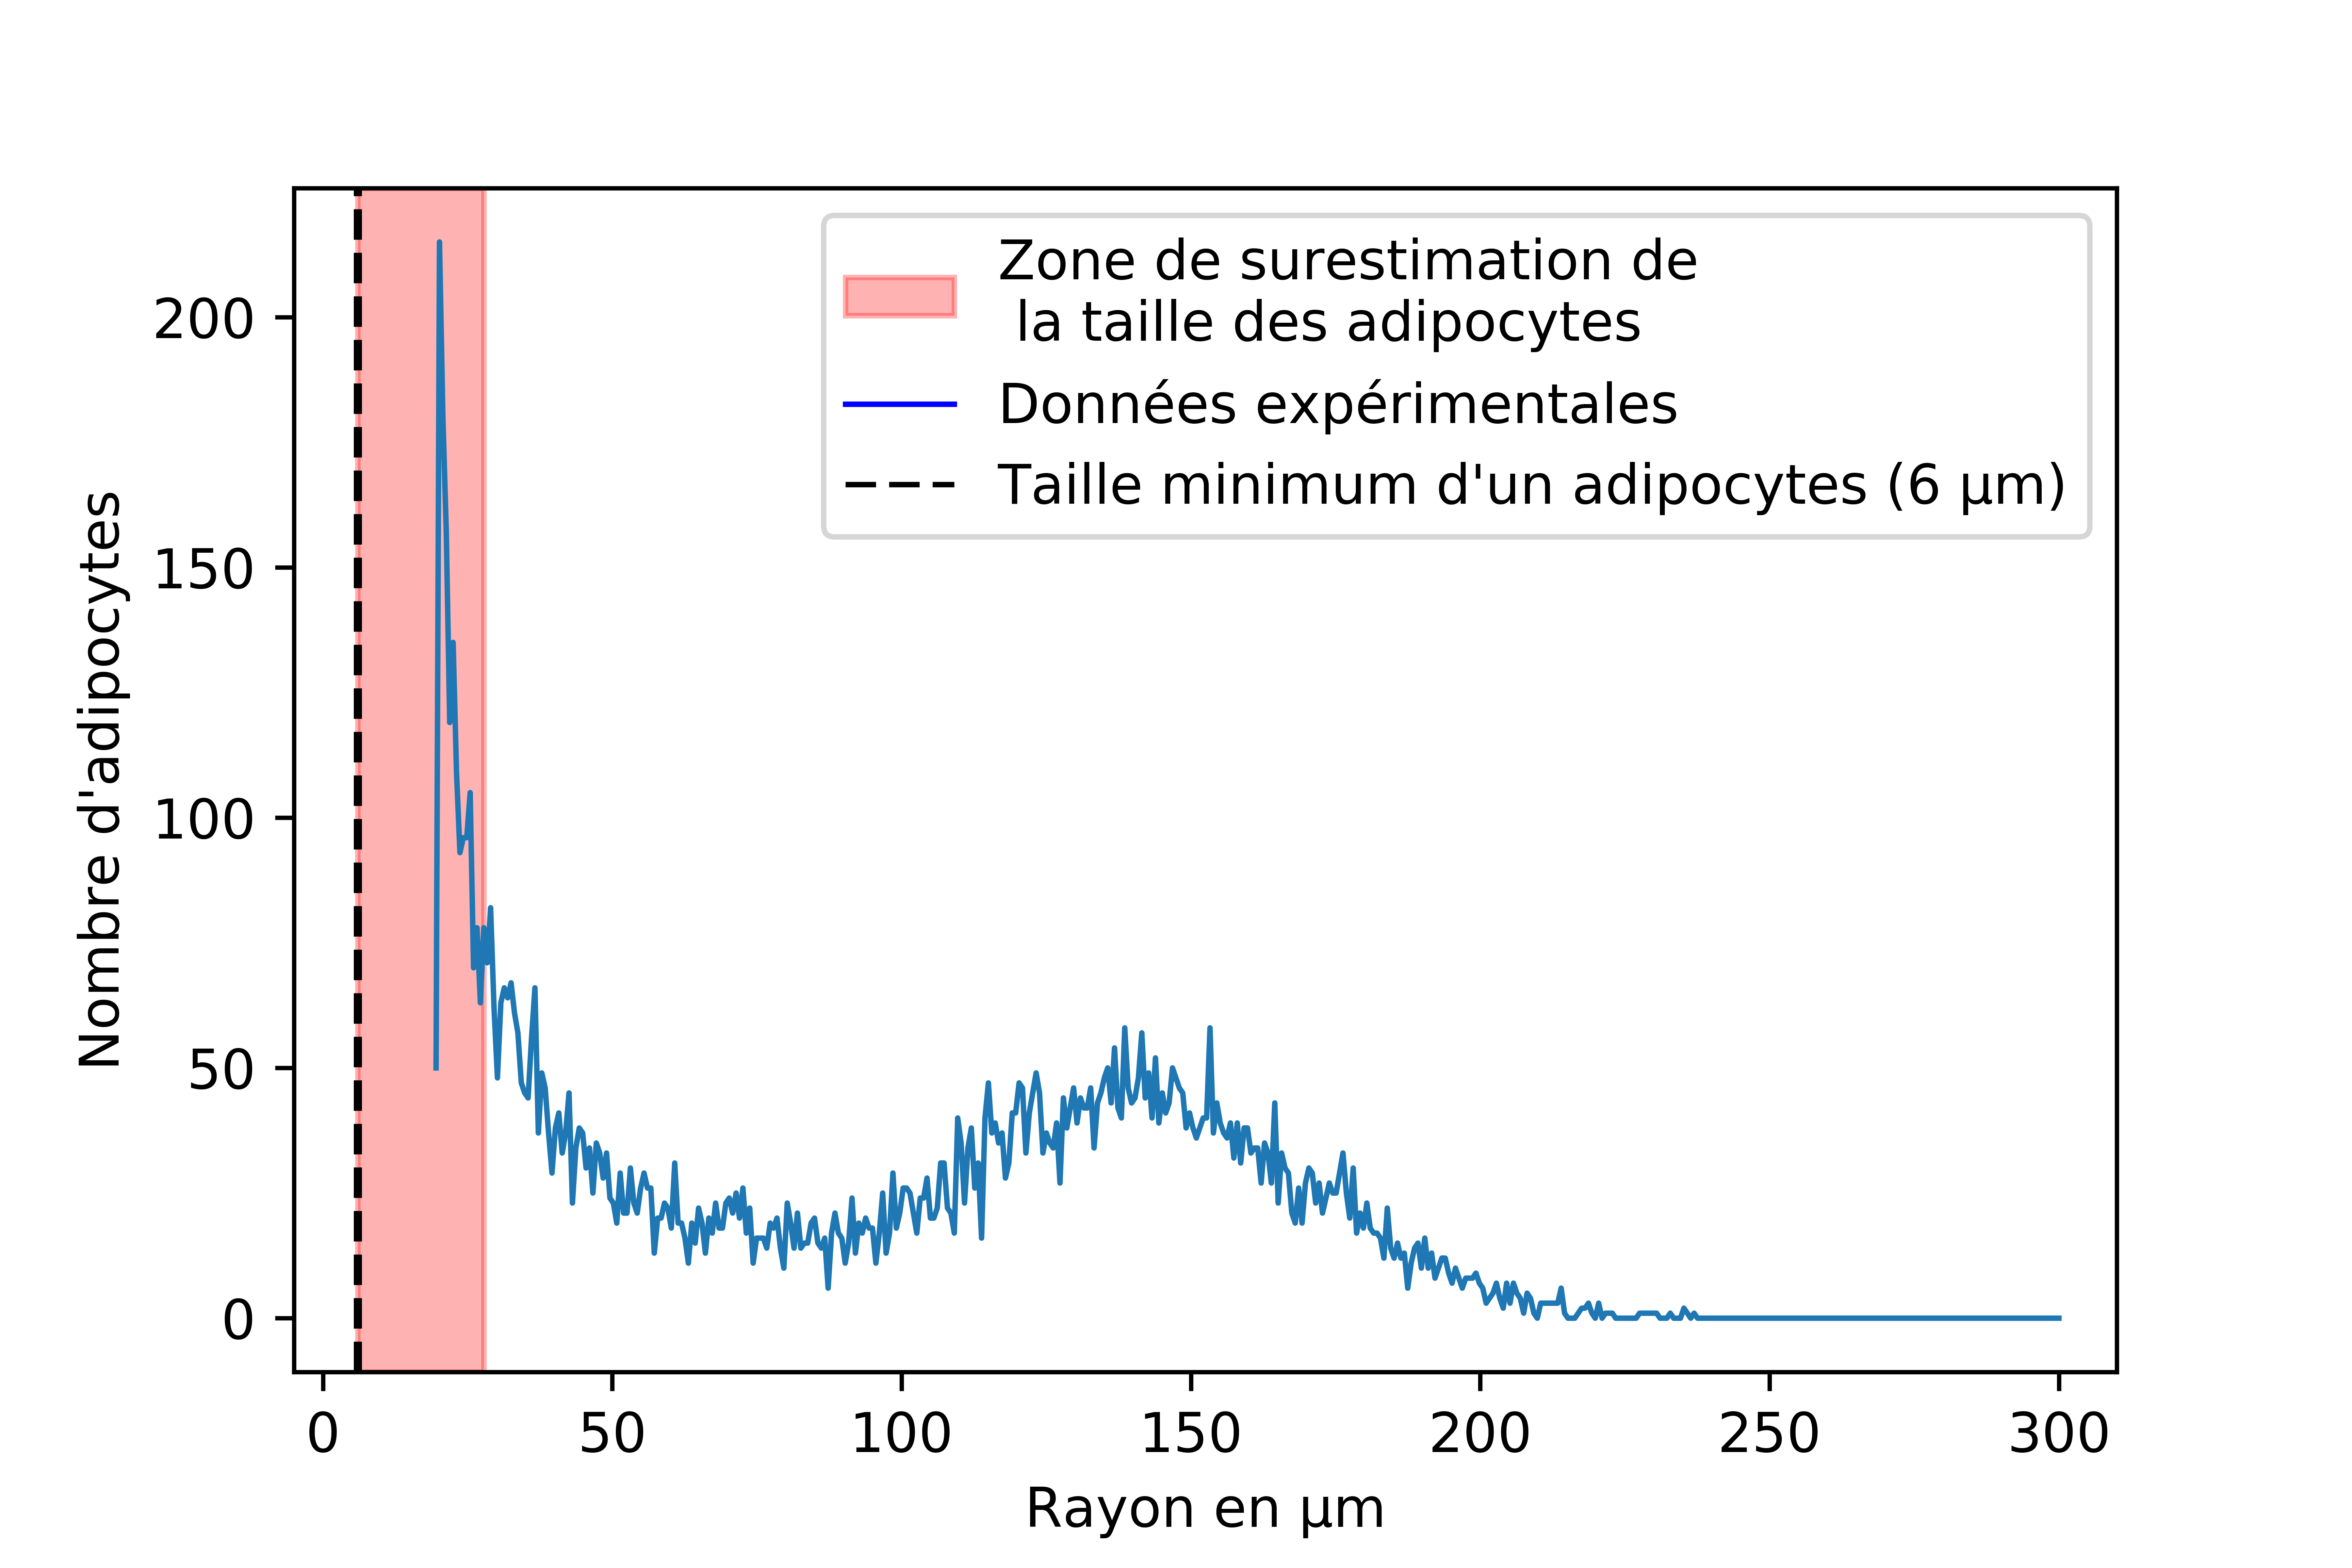
\includegraphics[scale=1]{data}
\caption{Illustration de la zone de surestimation de la taille des adipocytes sur une donnée expérimentale}
\label{figure:1}
\end{figure}


\subsection{Choix des paramètres à estimer et estimation sur des données synthétiques}

Avant de commencer à faire l'estimation sur données expérimentales, on doit choisir les paramètres à estimer et vérifier que notre méthode fonctionne sur des données synthétiques. Une donnée synthétique est obtenue à partir d'un jeu de paramètres donné, et est la distribution résultant d'une résolution du point fixe décrit plus haut.
 
Les paramètres que l'on peut faire varier dans notre problème sont : $a, B, b, \kappa_L, \kappa_r, n, \kappa_l, D$ et $L_{total} = L(0) + U(0)$. Les paramètres $B$, $b$ et $n$ ont été déterminés expérimentalement par conséquent on ne les estimera pas \cite{Soula2013}. On va donc travailler sur le jeu de paramètres : $\Theta = \{a,\kappa_r,\kappa_l,\kappa_L,D,L_{total}\}$.

Pour estimer notre jeu de paramètres, on va utiliser la méthode des moindres carrés. On dispose d'une distribution cible $u_{data}$ et on va chercher le jeu de paramètres $\Theta_{min}$ tel que la solution du point fixe associée $u_{\Theta_{min}}$ vérifie :
\[ \lVert u_{\Theta_{min}} - u_{data} \rVert_2 = \min_\Theta \lVert u_{\Theta} - u_{data} \rVert_2 \]

Pour chaque $\Theta$, on détermine $u_\Theta$ de la façon suivante : on trouve $L^{\infty}_\Theta$ comme solution du point fixe puis on calcul $u_\Theta$ à partir de $L^{\infty}_\Theta$.
On utilise ensuite la méthode \textit{scipy.optimize.minimize} qui minimise la distance avec la méthode de Nelder-Mead\cite{Nelder}.

Dans un premier temps, on vérifie que notre méthode fonctionne en l'appliquant sur une donnée synthétique. En partant d'une estimation mauvaise de $\Theta_{min}$, on regarde si notre méthode parviens à retrouver $\Theta_{min}$. Pour se faire, on choisis $\Theta_0$ le jeu de paramètres utilisé pour le schéma numérique (car on sait qu'il donnera une distribution bimodale) et on génère une suite $(\Theta_j)_{j=1}^{100}$ de la façon suivante : pour chaque paramètre de $\Theta_j$ on  une variable aléatoire uniforme sur $[0.8,1.2]$ que l'on multiplie par le paramètre en question. Ainsi $\forall j \leq 100, \Theta_j \in \bar{B}_{\mathbb{R}^6}(\Theta_0,0.2\Theta_0)$. On minimise alors la distance définie plus haut avec \textit{minimize} pour chaque $\Theta_j$ et avec l'estimation de départ $\Theta_0$. Chacun des $\Theta_j$ est alors assez peu éloigné de $\Theta_0$ et celui-ci doit donc être une bonne estimation de départ pour notre méthode. 
Le tableau 1 représente l'erreur relative moyenne entre le résultat de \textit{minimize} et $\Theta_j$ pour une donnée synthétique bruitée et non bruitée. Le bruit est ajouté à chaque point par la réalisation d'une loi Normale centrée réduite multipliée par un facteur qui donne un bruit du même ordre que la donnée expérimentale (dans notre cas 0.02).

\begin{figure}[H]
\centering
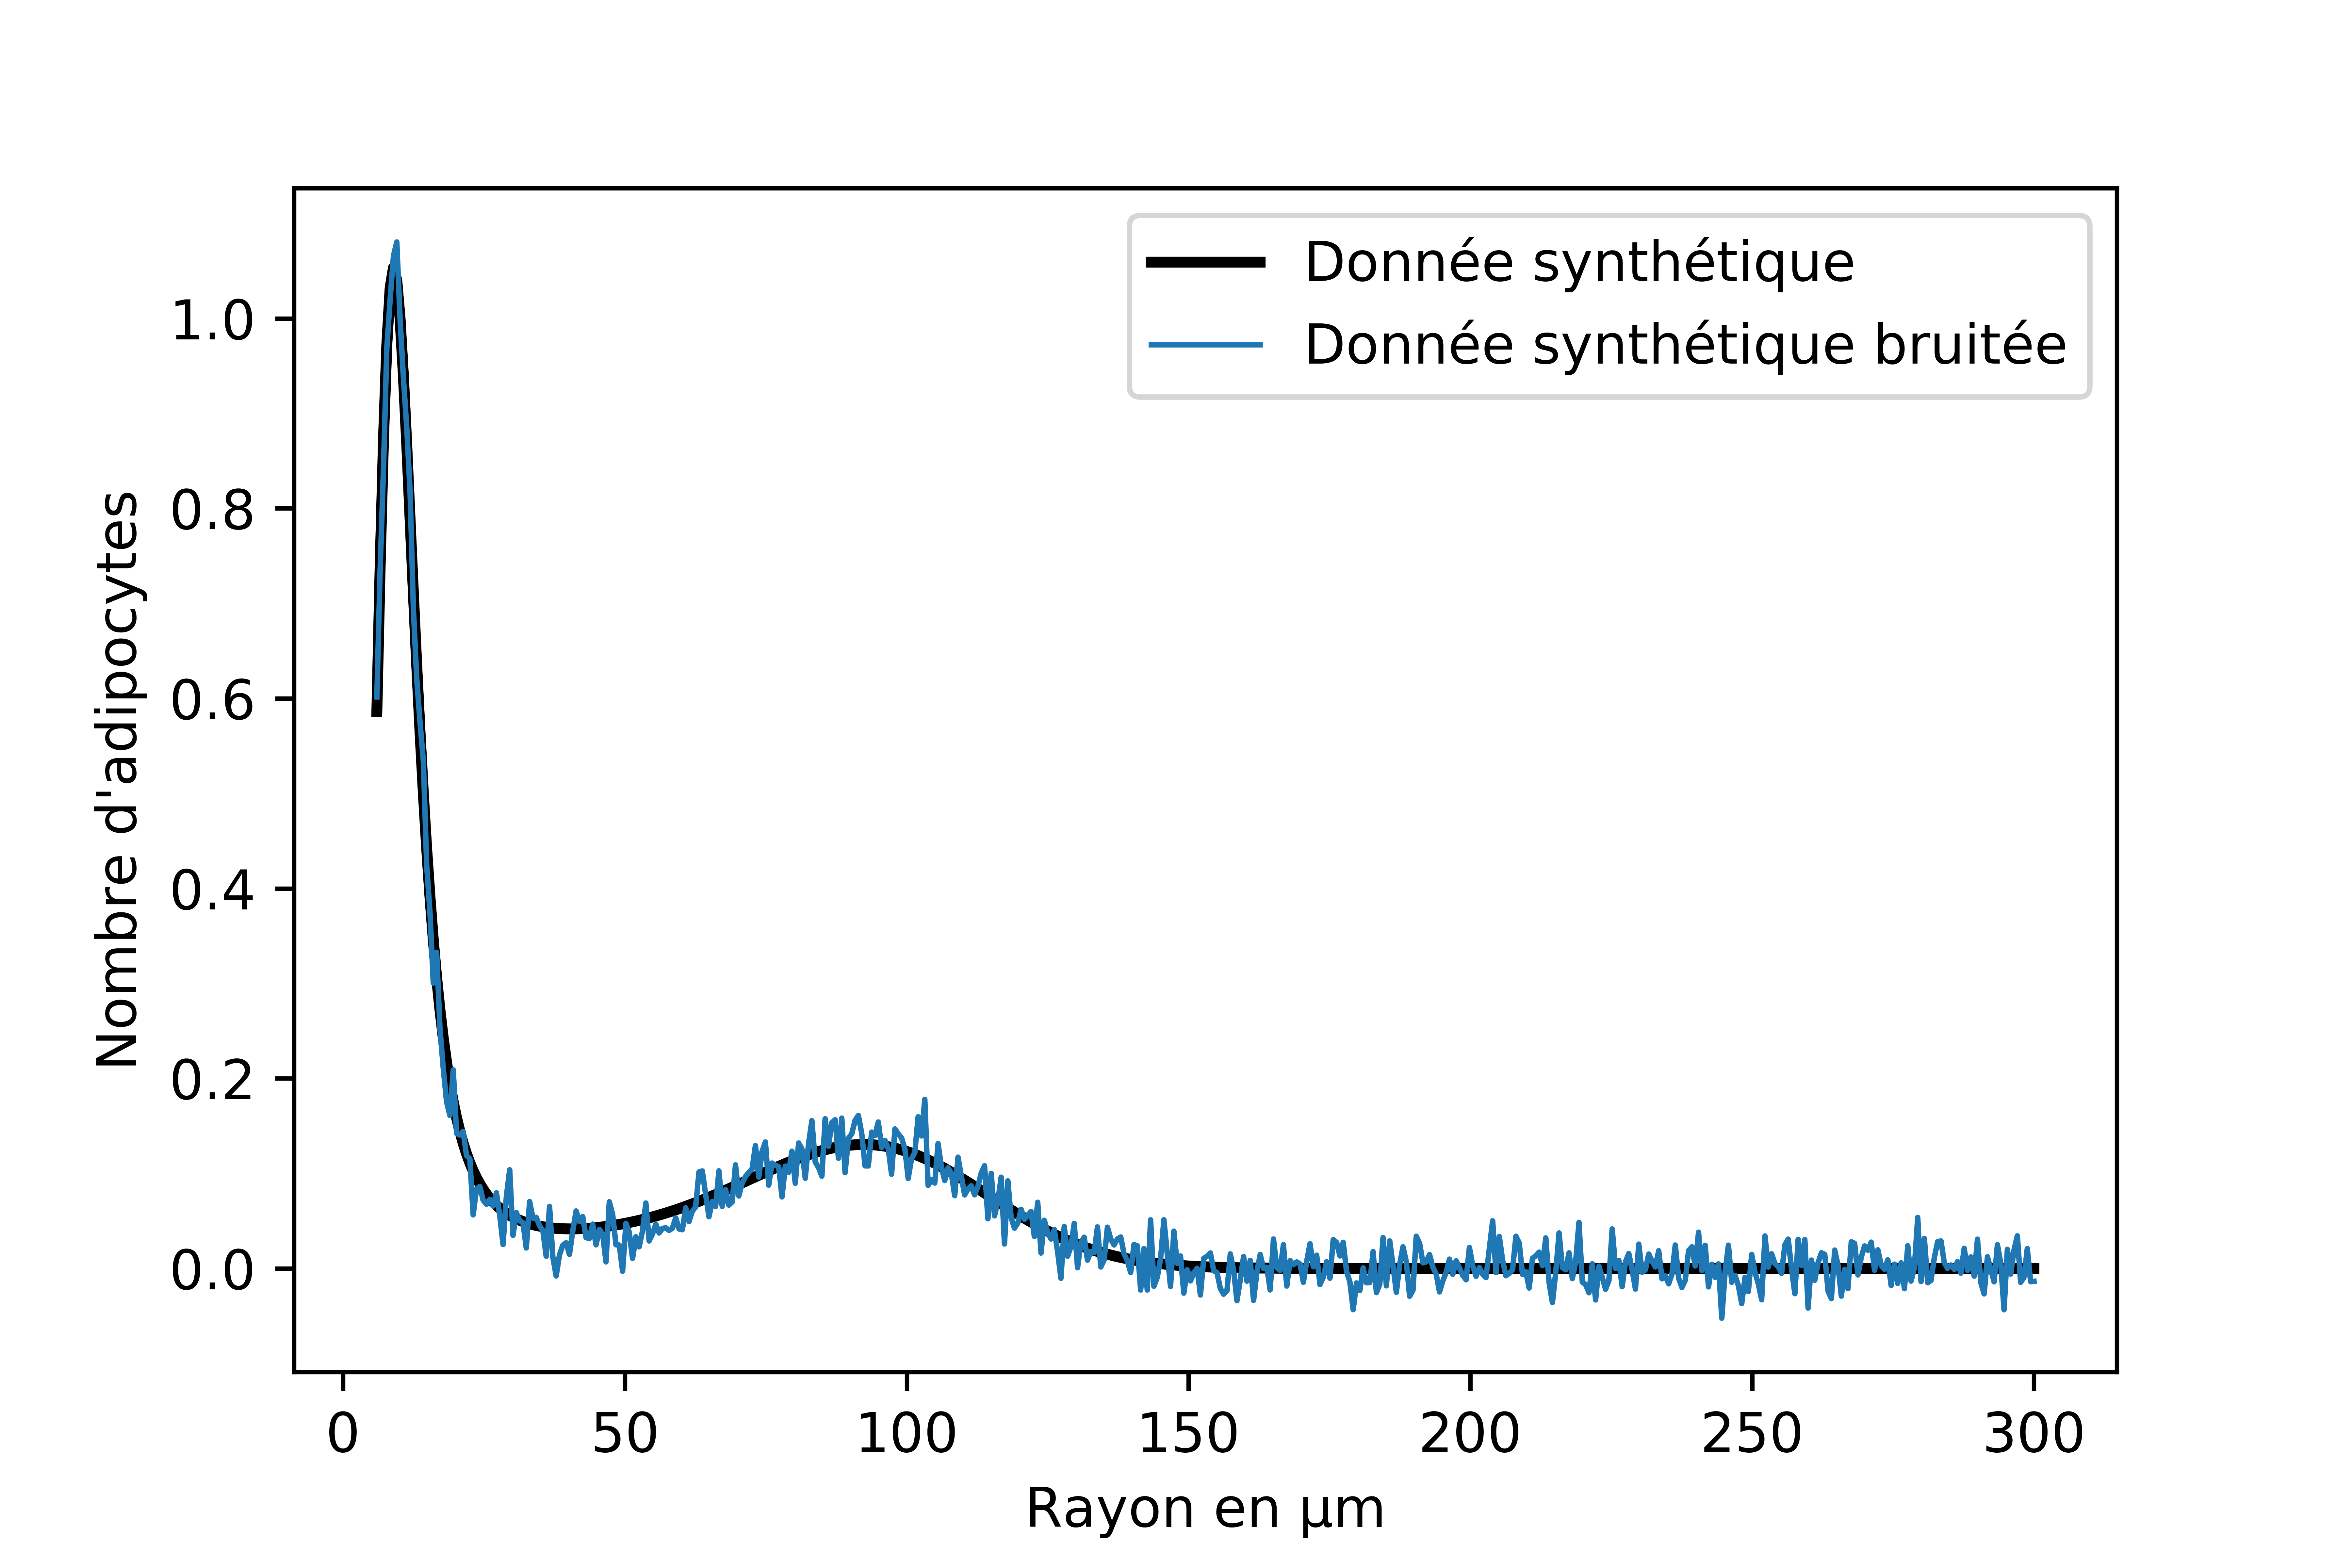
\includegraphics[scale=0.8]{synth}
\caption{Exemple de données synthétiques bruitée et non bruitée}
\label{figure:2}
\end{figure}

\begin{figure}[H]
\centering
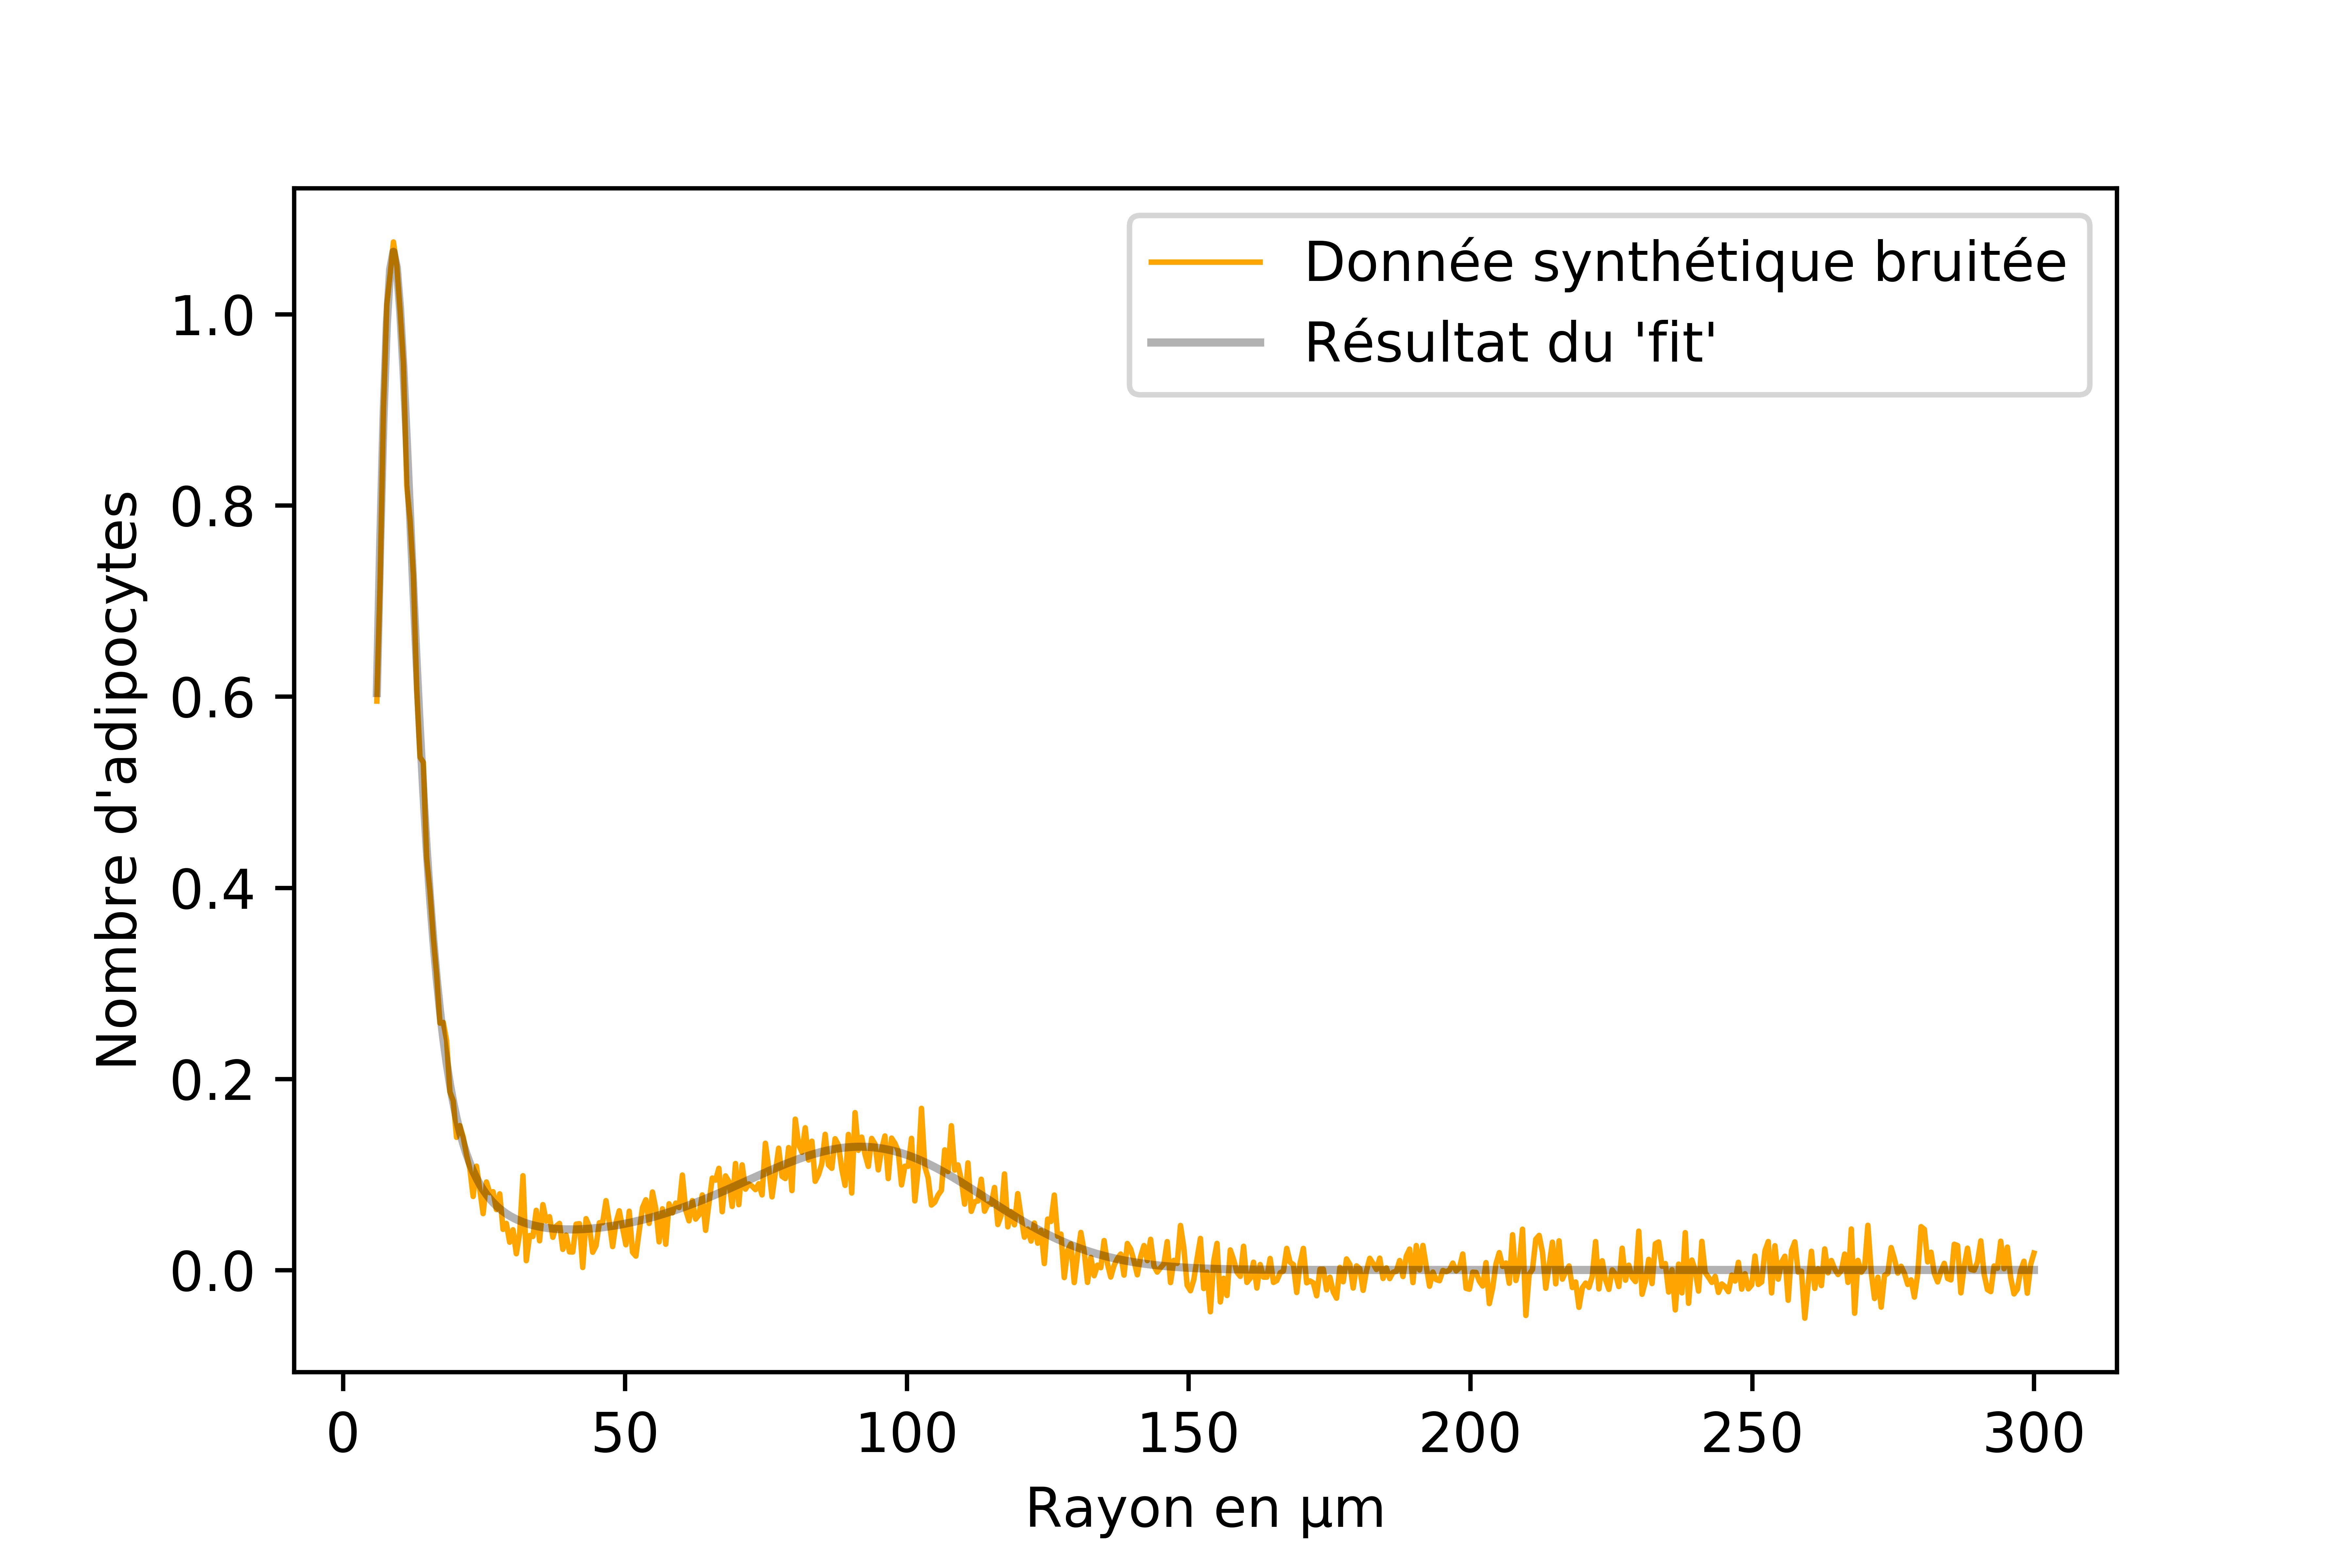
\includegraphics[scale=0.8]{fit_exemple}
\caption{Résultat d'un 'fit' sur une donnée synthétique bruitée}
\label{figure:3}
\end{figure}

\begin{table}[H]
\centering
\begin{tabular}{|c|c|c|}
\hline
Paramètres   & Donnée non bruitée & Donnée bruité\\
\hline
$a$         & $\simeq 7.8\%$ & $\simeq 9.0\%$\\
$K_r$       & $\leq 10^{-9}$ & $\simeq 1.2\%$\\
$K_l$       & $\leq 10^{-9}$ & $\simeq 1.2\%$\\
$K_L$       & $\simeq 7.0\%$ & $\simeq 8.5\%$\\
$D$         & $\leq 10^{-9}$ & $\simeq 1.8\%$\\
$L_{total}$ & $\simeq 0.8\%$ & $\simeq 4.0\%$\\
\hline
\end{tabular}
\caption{Erreur relative moyenne après 100 simulations. Pour chaque paramètre l'erreur est calculée de la façon suivante : $error = \dfrac{q-p}{p}$, où $p$ désigne la valeur du paramètre qui sert à générer la donnée synthétique et $q$ est la valeur du paramètre comme résultat du 'fit'.} 
\label{table : 1}
\end{table}

On remarque donc que \textit{minimize} parvient à retrouver les paramètres $K_r, K_l$ et $D$ mais commet une erreur sur $a, K_L$ et $L_{Ltotal}$. Il est donc probable que le problème soit sur-contraint. Cependant si on fixe, un des trois paramètres qui ont des erreurs significatives, on continue d'avoir ce type d'erreur sur les deux autres paramètres. Il est donc probable que pour certains jeux de données, il est plus difficile de trouver un minimum localement. Comme on ne peut pas prédire le jeu de paramètres correspondant à une donnée expérimentale, j'ai fait le choix de continuer d'estimer les six paramètres.

\newpage

\subsection{Estimation sur des données expérimentales}

On dispose de données expérimentales provenant de biopsies chez le rat. Ces données ont une surestimation du nombre de petits adipocytes car l'appareil de mesure a une borne inférieure de détection, une partie des adipocytes sont donc de taille inférieure à cette borne mais ont un rayon surévalué dans les données. On va donc intégrer cette information en supposant qu'un pourcentage de cellules se trouve sous cette borne inférieure de mesure. Ce pourcentage ne correspond pas à au pourcentage de cellules observées sous la borne mais représente une estimation de cellules sous cette borne, qu'elles aient été comptées ou non. On va donc normaliser nos données en conséquence.
On note $M_{data}$ le nombre de cellules de nos données et $X$ ce pourcentage. On cherche donc $\lambda$ tel que :
\[\dfrac{M_{data}}{\lambda} + X = 1 \Rightarrow \lambda = \dfrac{M_{data}}{1 - X}\]
On fait donc une estimation avec une masse totale de 1 et sur la donnée normalisée $\dfrac{u_{data}}{\lambda}$. Pour s'assurer que l'on fais notre estimation seulement sur les données dont on dispose, on ne calcule la norme $\lVert \cdot \rVert_2$ que sur l'intervalle où on a des données : on choisit $r_{data} \geq r_{min}$ tel que $u_{data}(r_{data}) \neq 0$ et on calcule la norme sur $[r_{data},r_{max}]$. De plus on introduit un seuil minimum pour le rayon, car les adipocytes ont une taille minimum, on choisit la taille moyenne d'un noyau cellulaire chez les mammifères : 6 $\mu$m \cite{Cell}.

Comme les données expérimentales sont assez différentes, il semble compliqué de fixer un $\lambda$ et un $r_{data}$ commun à toutes les données. On va donc rajouter $\lambda$ et $r_{data}$ comme paramètre du 'fit' pour chaque donnée. Comme estimation de départ on prendra 20\% pour $\lambda$ et $min\{r | u_{data}(r) \neq 0\}$ pour $r_{data}$.

\begin{figure}[H]
\centering
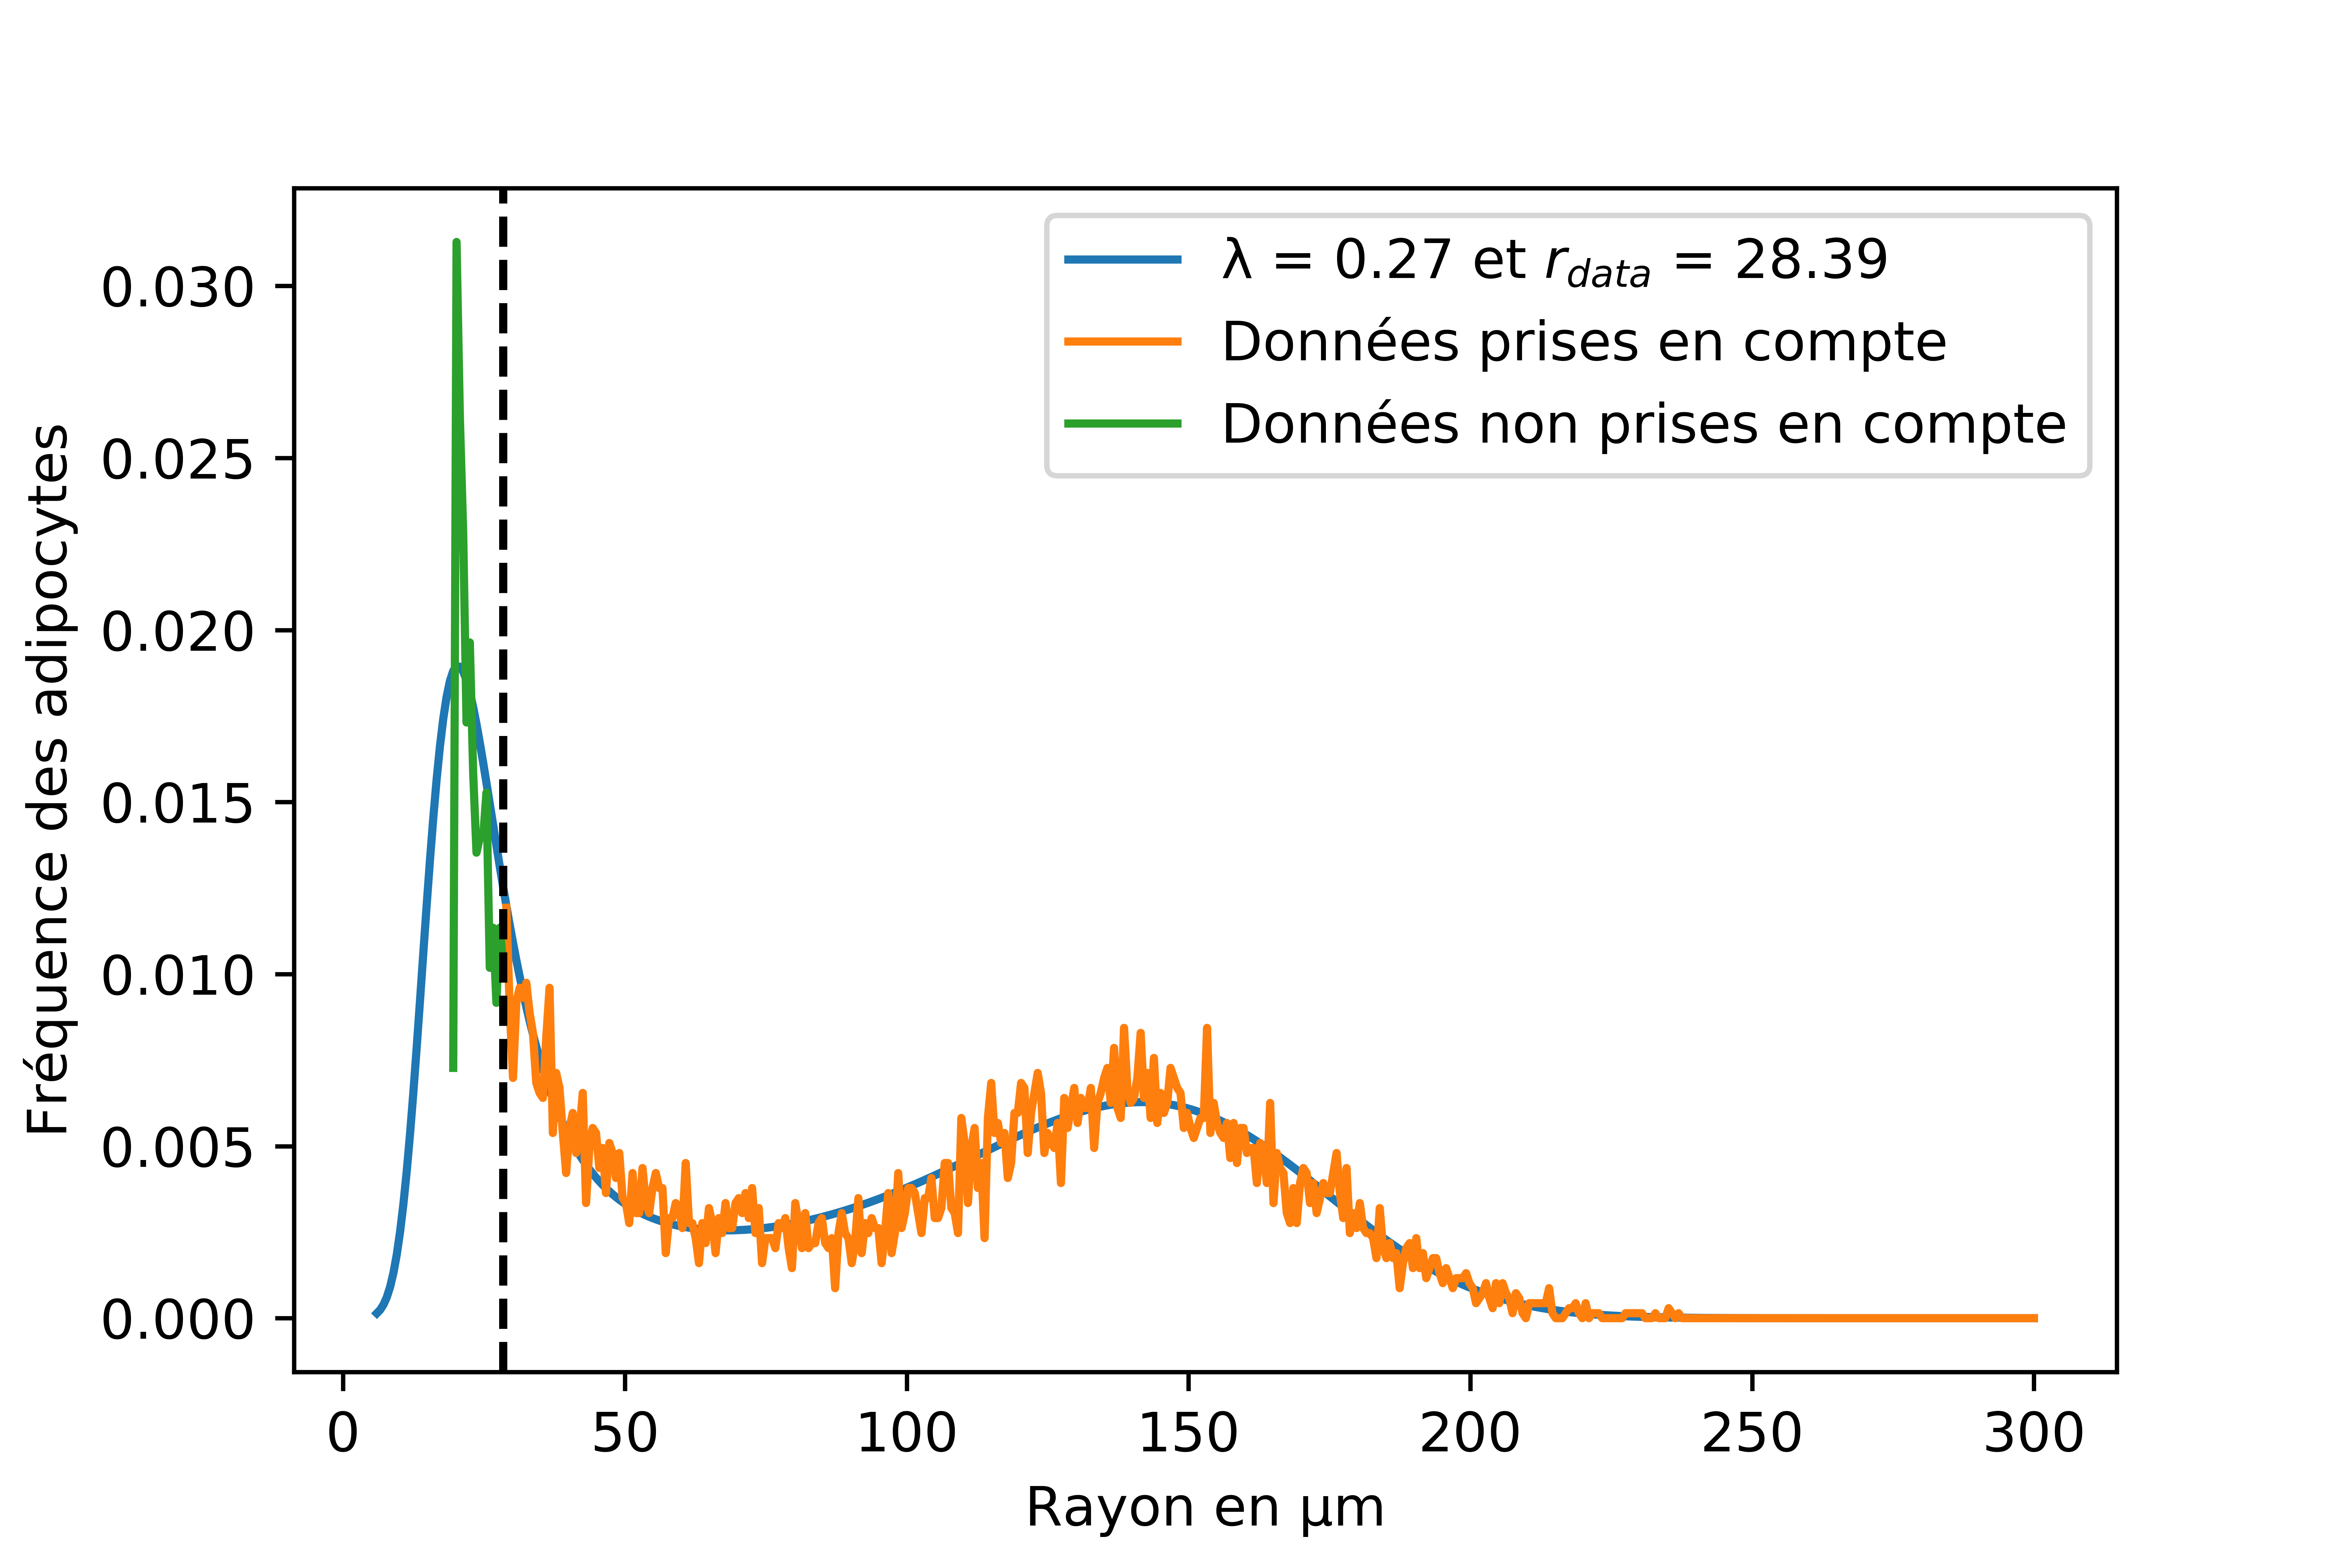
\includegraphics[scale=1]{Hys-D0-5-1}
\caption{Résultat d'un 'fit' sur une donnée expérimentale.}
\label{figure:4}
\end{figure}

Dans l'annexe \ref{appendix:A}, sont présentés des résultats de 'fitting' sur d'autres données expérimentales. On remarque qu'en général, on arrive à retrouver les 2 modes mais pas le nadir qui est sous-estimé. Également, on observe que le paramètre $\lambda$ est souvent élevé (supérieur à 30\%), ce qui donne un premier mode largement supérieur au second, indiquant qu'on ne parviens pas totalement à faire disparaître la surestimation du nombre de petit adipocyte par l'appareil de mesure. Pour palier à ces effets, il serait intéressant de faire une étude de la sensibilité de chaque paramètre sur les 2 modes et le nadir afin d'affiner pour chaque donnée expérimentale notre estimation de départ pour le 'fit'.

\subsection{Approximate Bayesian Computation}

\subsubsection{Un premier algorithme}

Comme notre problème de minimisation semble sur-contraint, on va chercher la distribution postérieure des paramètres qui présentent une erreur significative ($a, K_L,L_{total}$) avec la méthode ABC : Approximate Bayesian Computation. L'idée est la suivante : on dispose d'une donnée $u_{data}$ et pour chaque paramètre, on cherche la distribution des valeurs qui permettent d'approcher $u_{data}$ à un seuil $\varepsilon$ près.

L'algorithme est le suivant :
\begin{itemize}
\item On génère $\Theta_i, 1<i<N$ selon une distribution antérieur, ici on choisit une distribution uniforme pour chaque paramètre;
\item On calcul $u_{\Theta_i}$ et si $\lVert u_{\Theta_i} - u_{data}\rVert_2 < \varepsilon$, on garde $\Theta_i$;
\item On affiche tout les $\Theta_i$ que l'on a conservé.
\end{itemize}


La figure \ref{figure:5} présente les résultats de l'algorithme précédent, avec $N=15000$ et $\varepsilon = 0.1$ pour les paramètres qui nous intéressent : $a, K_L,L_{total}$.

\begin{figure}[H]
\centering
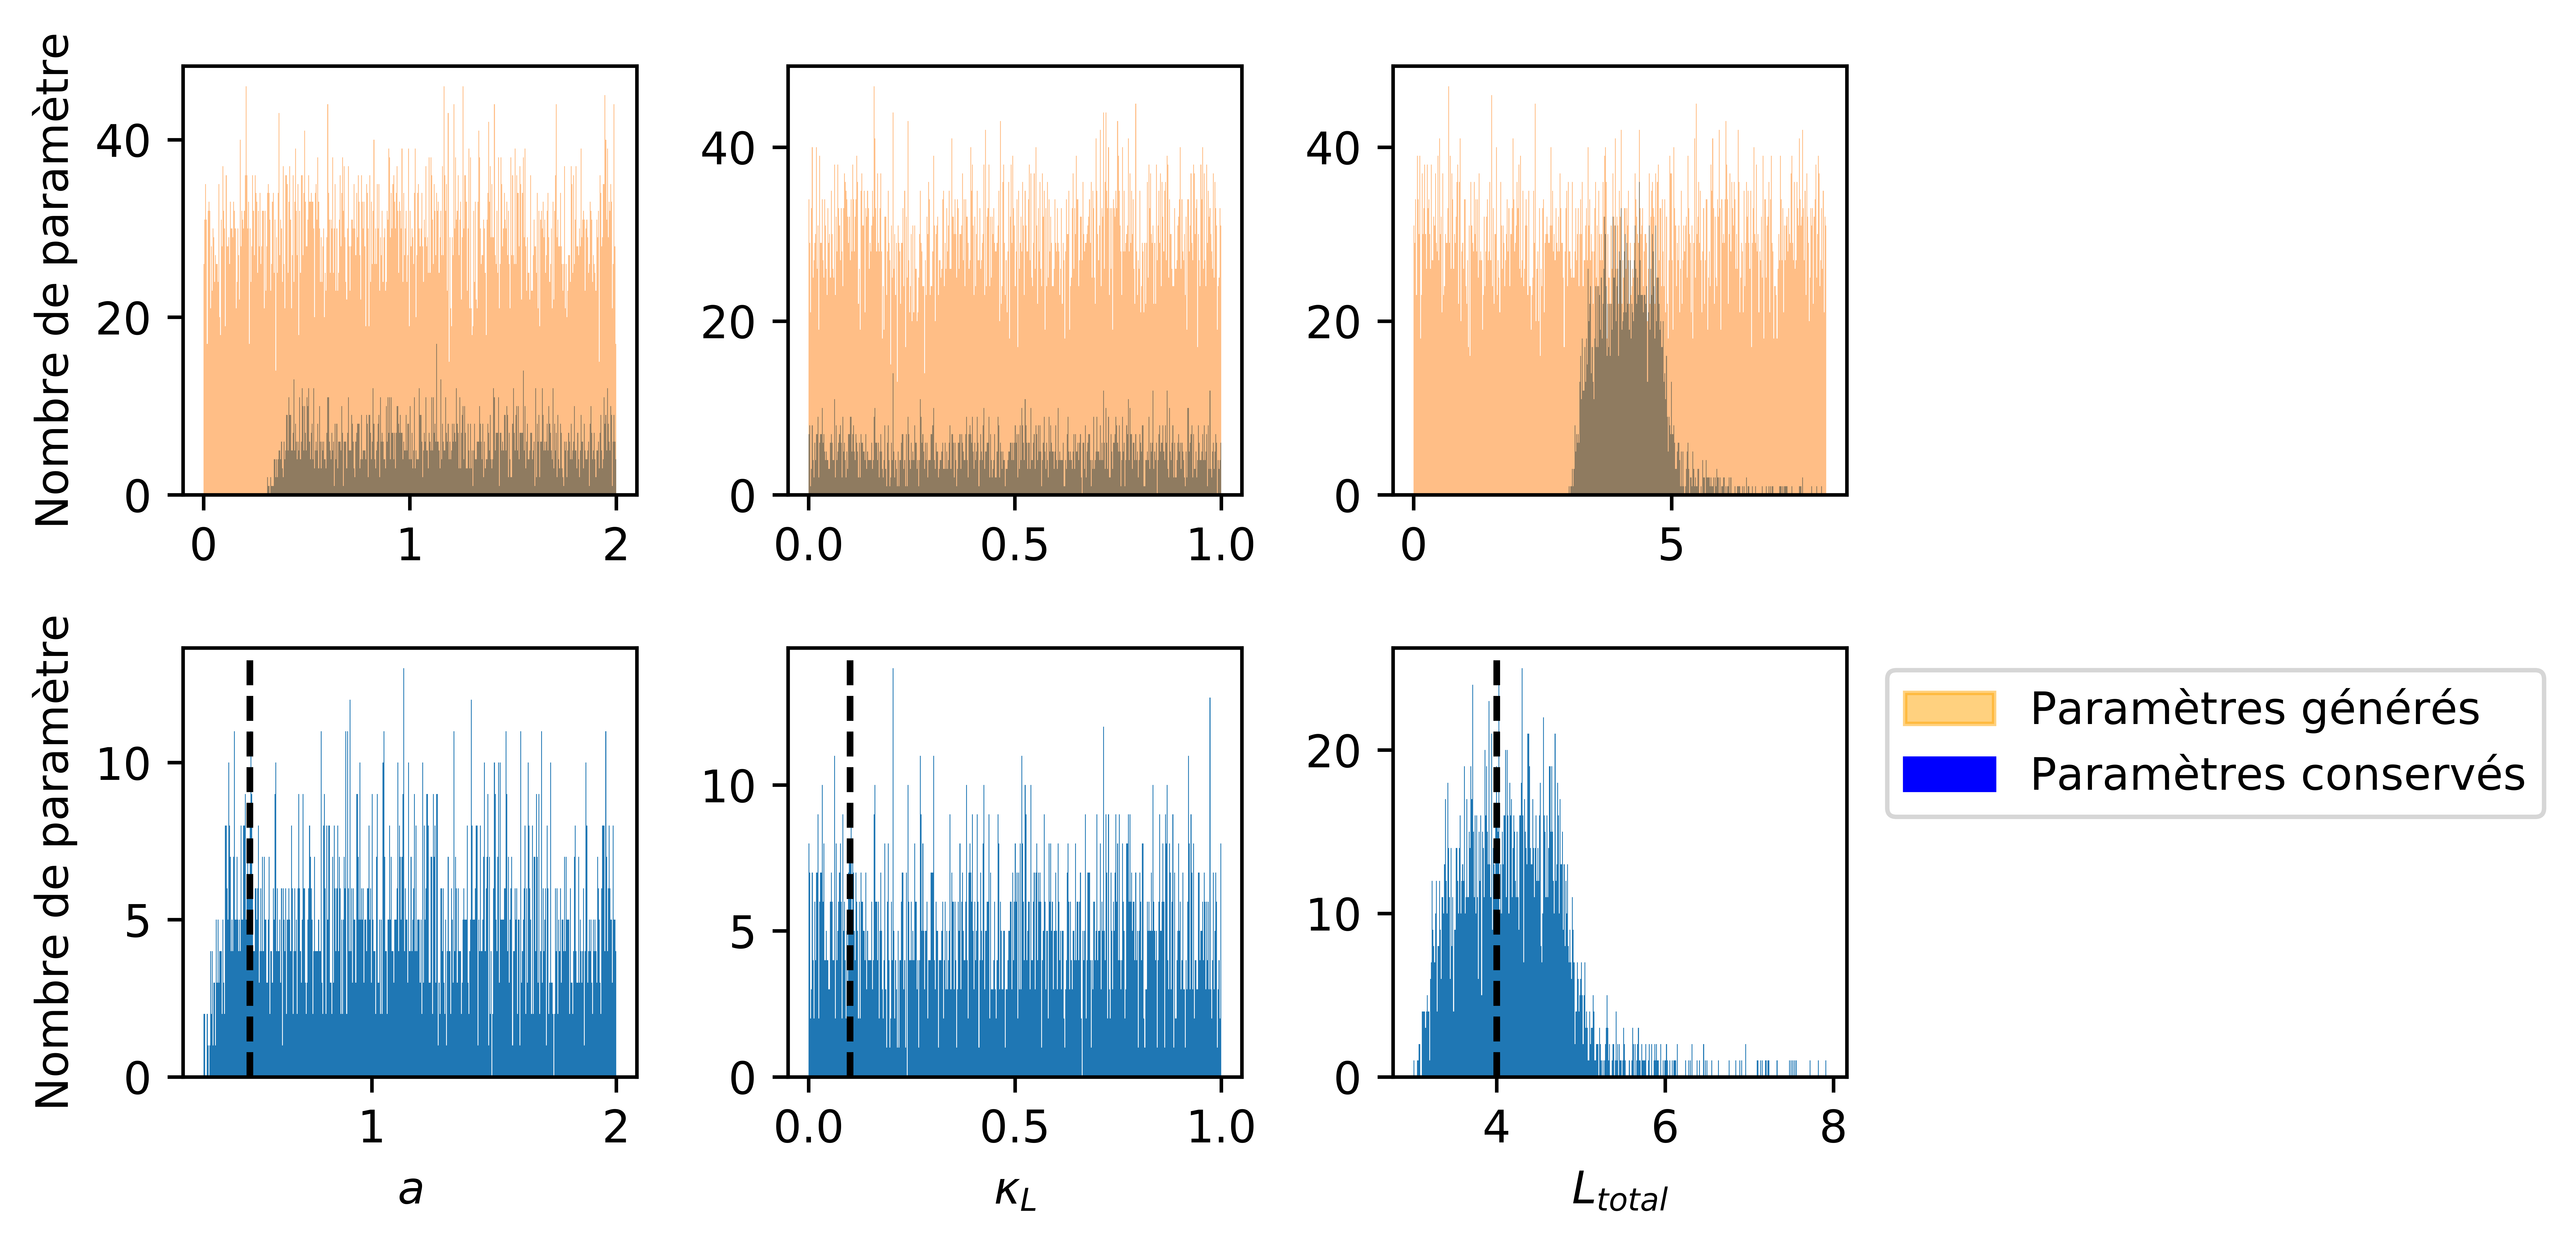
\includegraphics[scale=0.8]{abc_distrib}
\centering
\caption{Résultats de l'algorithme ABC présenté plus haut. La première ligne indique les paramètres générés et les paramètres conservés. La seconde présente seulement les paramètres conservés.}
\label{figure:5}
\end{figure}

On remarque que pour $L_{total}$ on a une distribution centrée autour de la valeur choisit pour générer $u_{data}$, cependant ce n'est pas le cas pour $a$ et $\kappa_L$ qui continue de suivre une distribution uniforme. Afin de vérifier si on ne peut pas affiner ces distributions en diminuant $\varepsilon$, on trace la norme $\lVert u_{\Theta_i} - u_{data}\rVert_2$ en fonction de chaque paramètre dans la figure \ref{figure:6}. Contrairement à $L_{total}$, on n'observe pas de paterne dans la répartition des normes pour $a$ et $\kappa_L$. Cela laisse nous indique que peu importe le seuil $\varepsilon$, on ne parviendra pas à améliorer la distribution postérieure de $a$ et $\kappa_L$. On va donc affiner notre méthode en utilisant un algorithme plus efficace : Population Monte Carlo Approximate Bayesian Computation.

\begin{figure}[H]
\centering
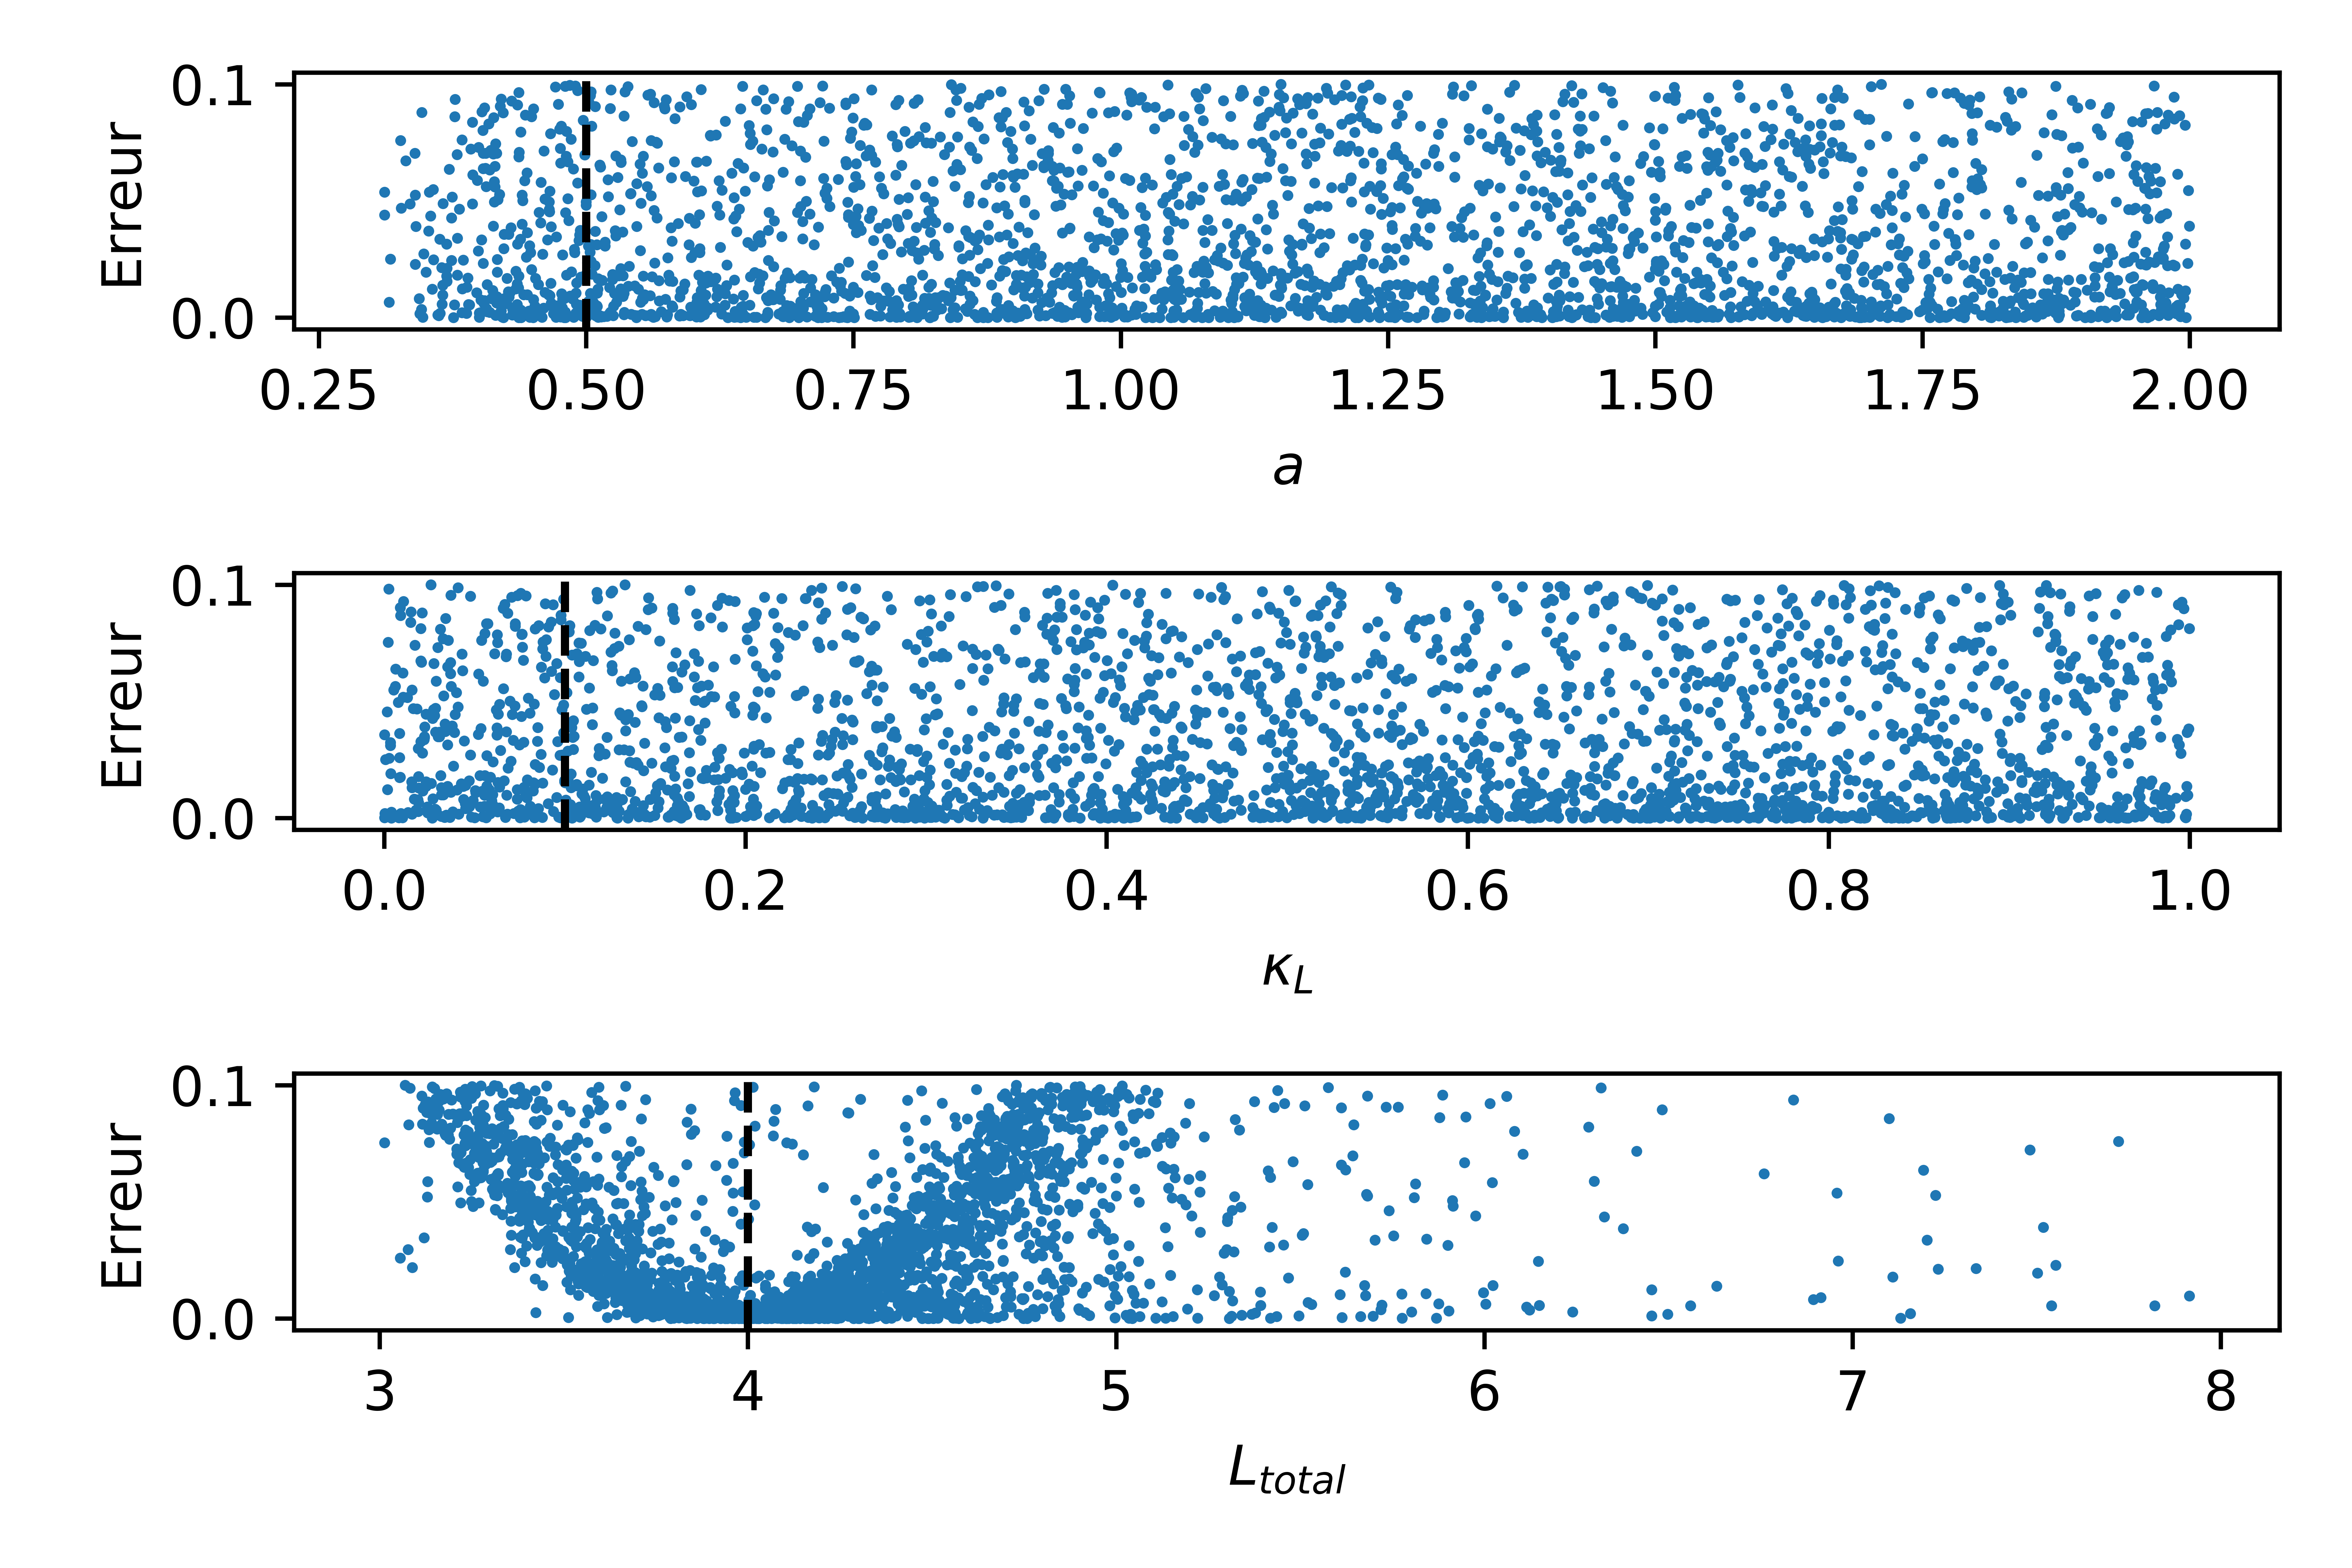
\includegraphics[scale=1]{abc_error}
\centering
\caption{Erreur pour chaque paramètre conservé dans l'algorithme ABC}
\label{figure:6}
\end{figure}

\subsubsection{Population Monte Carlo Approximate Bayesian Computation}

Afin d'affiner les distributions postérieures de nos paramètres, on va utiliser un algorithme ABC plus puissant : Population Monte Carlo Approximate Bayesian Computation (PMCABC). L'algorithme est décrit dans \cite{Beaumont} et j'ai utilisé le package Python \textit{abcpmc} qui l'implémente, décrit dans \cite{PMCABC}. Dans un premier temps, on regarde comme précédemment l'algorithme sur une donnée synthétique bruitée puis ensuite sur une donnée expérimentale.

Les résultats sur donnée synthétique sont présentés dans la figure \ref{figure:7}, et sur donnée expérimentale dans la figure \ref{figure:8}. On observe pour chaque paramètre une distribution semblable à une loi normale. Dans le tableau \ref{table : 2} sont présentés les écarts types pour chaque paramètre. On observe que pour chaque paramètre on obtient un coefficient de variation (écart-type divisé par la moyenne) similaire. Dans les deux cas, l'algorithme retrouve les paramètre de la donnée synthétique et du 'fit' pour la donnée expérimentale. Cependant comme il est difficile de retrouver un minimum local pour certains paramètres, comme vu plus haut, dans certains cas l'algorithme ne parvient pas à retrouver ces paramètres et commet une erreur. Un tel résultat est présenté dans l'annexe \ref{appendix:B}




\begin{figure}[H]
\centering
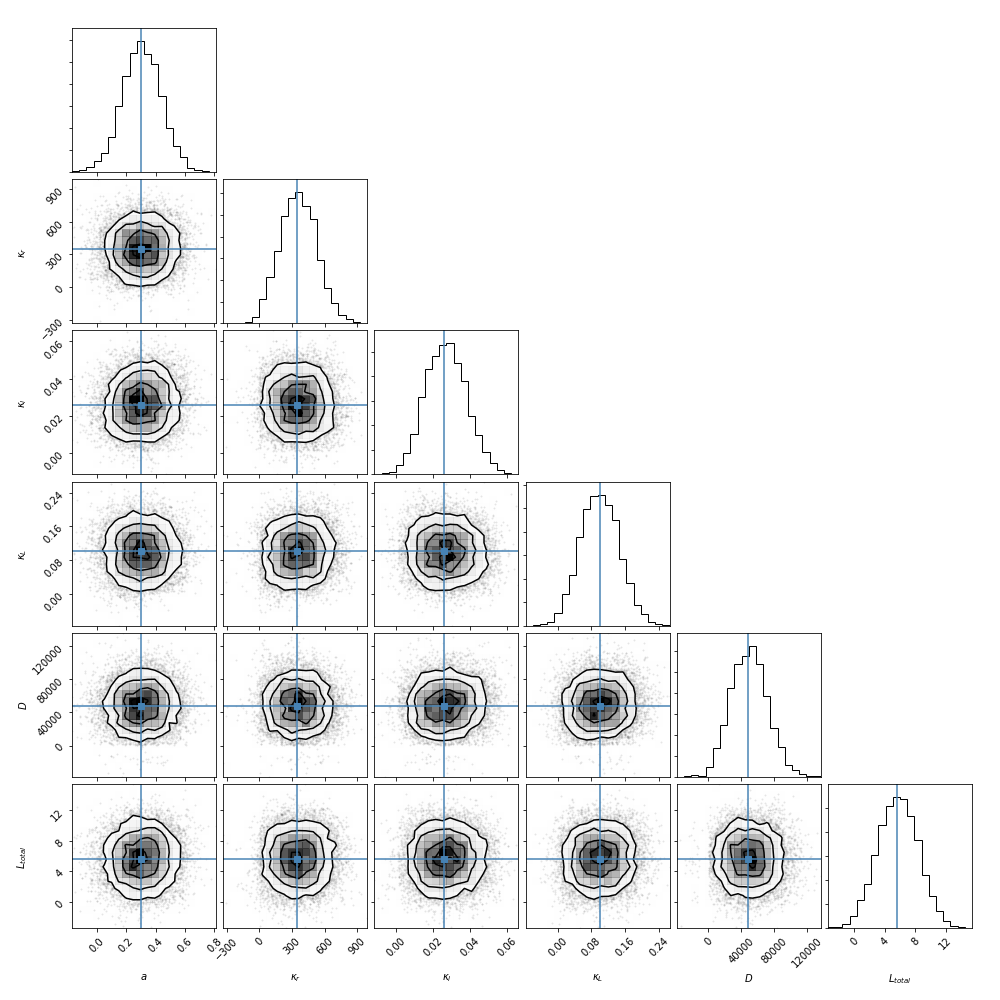
\includegraphics[scale=0.5]{abcpmc_synth}
\centering
\caption{Résultat de l'algorithme PMCABC sur une donnée synthétique. En bleu, les paramètres servant à générer la donnée synthétique.}
\label{figure:7}
\end{figure}


\begin{figure}[H]
\centering
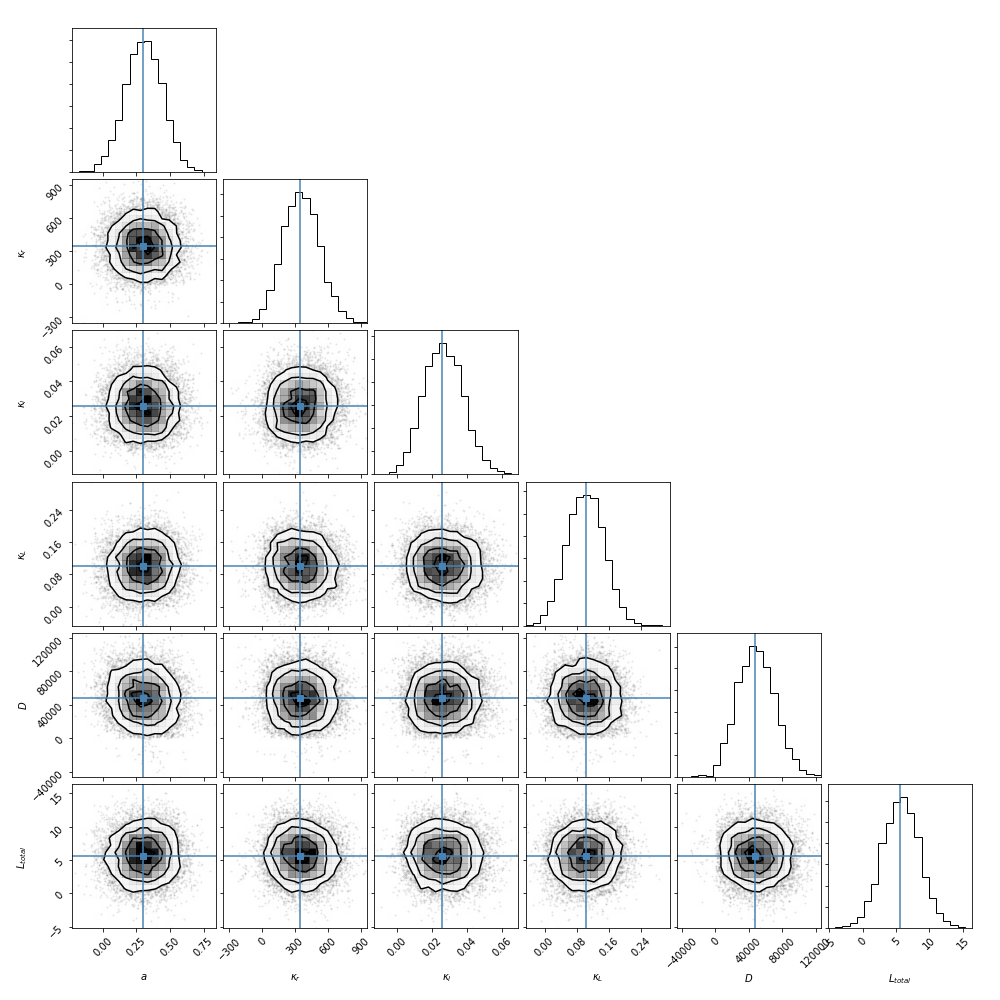
\includegraphics[scale=0.5]{abcpmc_data}
\centering
\caption{Résultat de l'algorithme PMCABC sur une donnée expérimentale. En bleu, les paramètres provenant du 'fit' avec la donnée expérimentale.}
\label{figure:8}
\end{figure}

\begin{table}[H]
\centering
\begin{tabular}{|c|c|c|}
\hline
Paramètres   & Donné synthétique & Donnée expérimentale\\
\hline
$a$         & 0.4329 & 0.4555\\
$K_r$       & 0.4696 & 0.4727\\
$K_l$       & 0.4098 & 0.4238\\
$K_L$       & 0.4549 & 0.4462\\
$D$         & 0.4418 & 0.4576\\
$L_{total}$ & 0.4593 & 0.4826\\
\hline
\end{tabular}
\caption{Coefficient de variation pour chaque paramètre après un algorithme PMCABC, pour une donnée synthétique et une donnée expérimentale.} 
\label{table : 2}
\end{table}

\section{Conclusion}

En conclusion, pendant ce stage j'ai approché trois sujet autour du modèle de la distribution des adipocytes : les schémas numériques, les solutions stationnaires et l'estimation de paramètres.

Concernant les schémas numériques, l'ajout d'un schéma de Cranck-Nicolson pour la partie diffusive a permis d'impliciter le schéma. Cela a notamment réduit le temps de calcul, mais comme à chaque pas de temps, on doit résoudre un système linéaire de dimension $J$, l'algorithme est plus complexe. On pourrait perdre ce gain de temps pour certains jeux de paramètres ou certaines conditions initiales.

A propos des solutions stationnaires, la relation entre la convergence du schéma numérique vers une solution stationnaire et l'attractivité du point fixe n'est pas forcément établit. J'ai notamment considéré qu'il n'existait qu'un seul point fixe positif mais il pourrait en exister plusieurs et donc plusieurs solutions stationnaires. Également, comme on a une hypothèse de conservation de la masse, il serait intéressant d'étudier comment la masse influe sur la solution stationnaire.

Enfin concernant l'estimation de paramètres, j'ai rencontré quelques difficultés liées au fait que l'espace d'état de nos paramètres est très hétérogène par rapport au résultat de la minimisation. En effet, il semble que certains jeux de paramètres soient plus ou moins difficile à retrouver par minimisation et/ou que plusieurs jeux donnent une même distribution. Même si les algorithmes ABC nous ont apporté quelques informations, je pense qu'elles restent très spécifique au jeu de paramètres choisis. Dans ce sens, il me semble intéressant de faire des analyses de sensibilité pour les paramètres. Particulièrement sur le résultat du point fixe mais aussi sur les modes et le nadir des solutions stationnaires.

Pour terminer sur une pointe d'humour, je citerais Karadoc dans Kaamelott : "Le gras, c'est la vie".


\newpage

\appendix

\section{Quelques résultats de 'fit' sur donnée expérimentale}\label{appendix:A}

\begin{figure}[H]
\centering
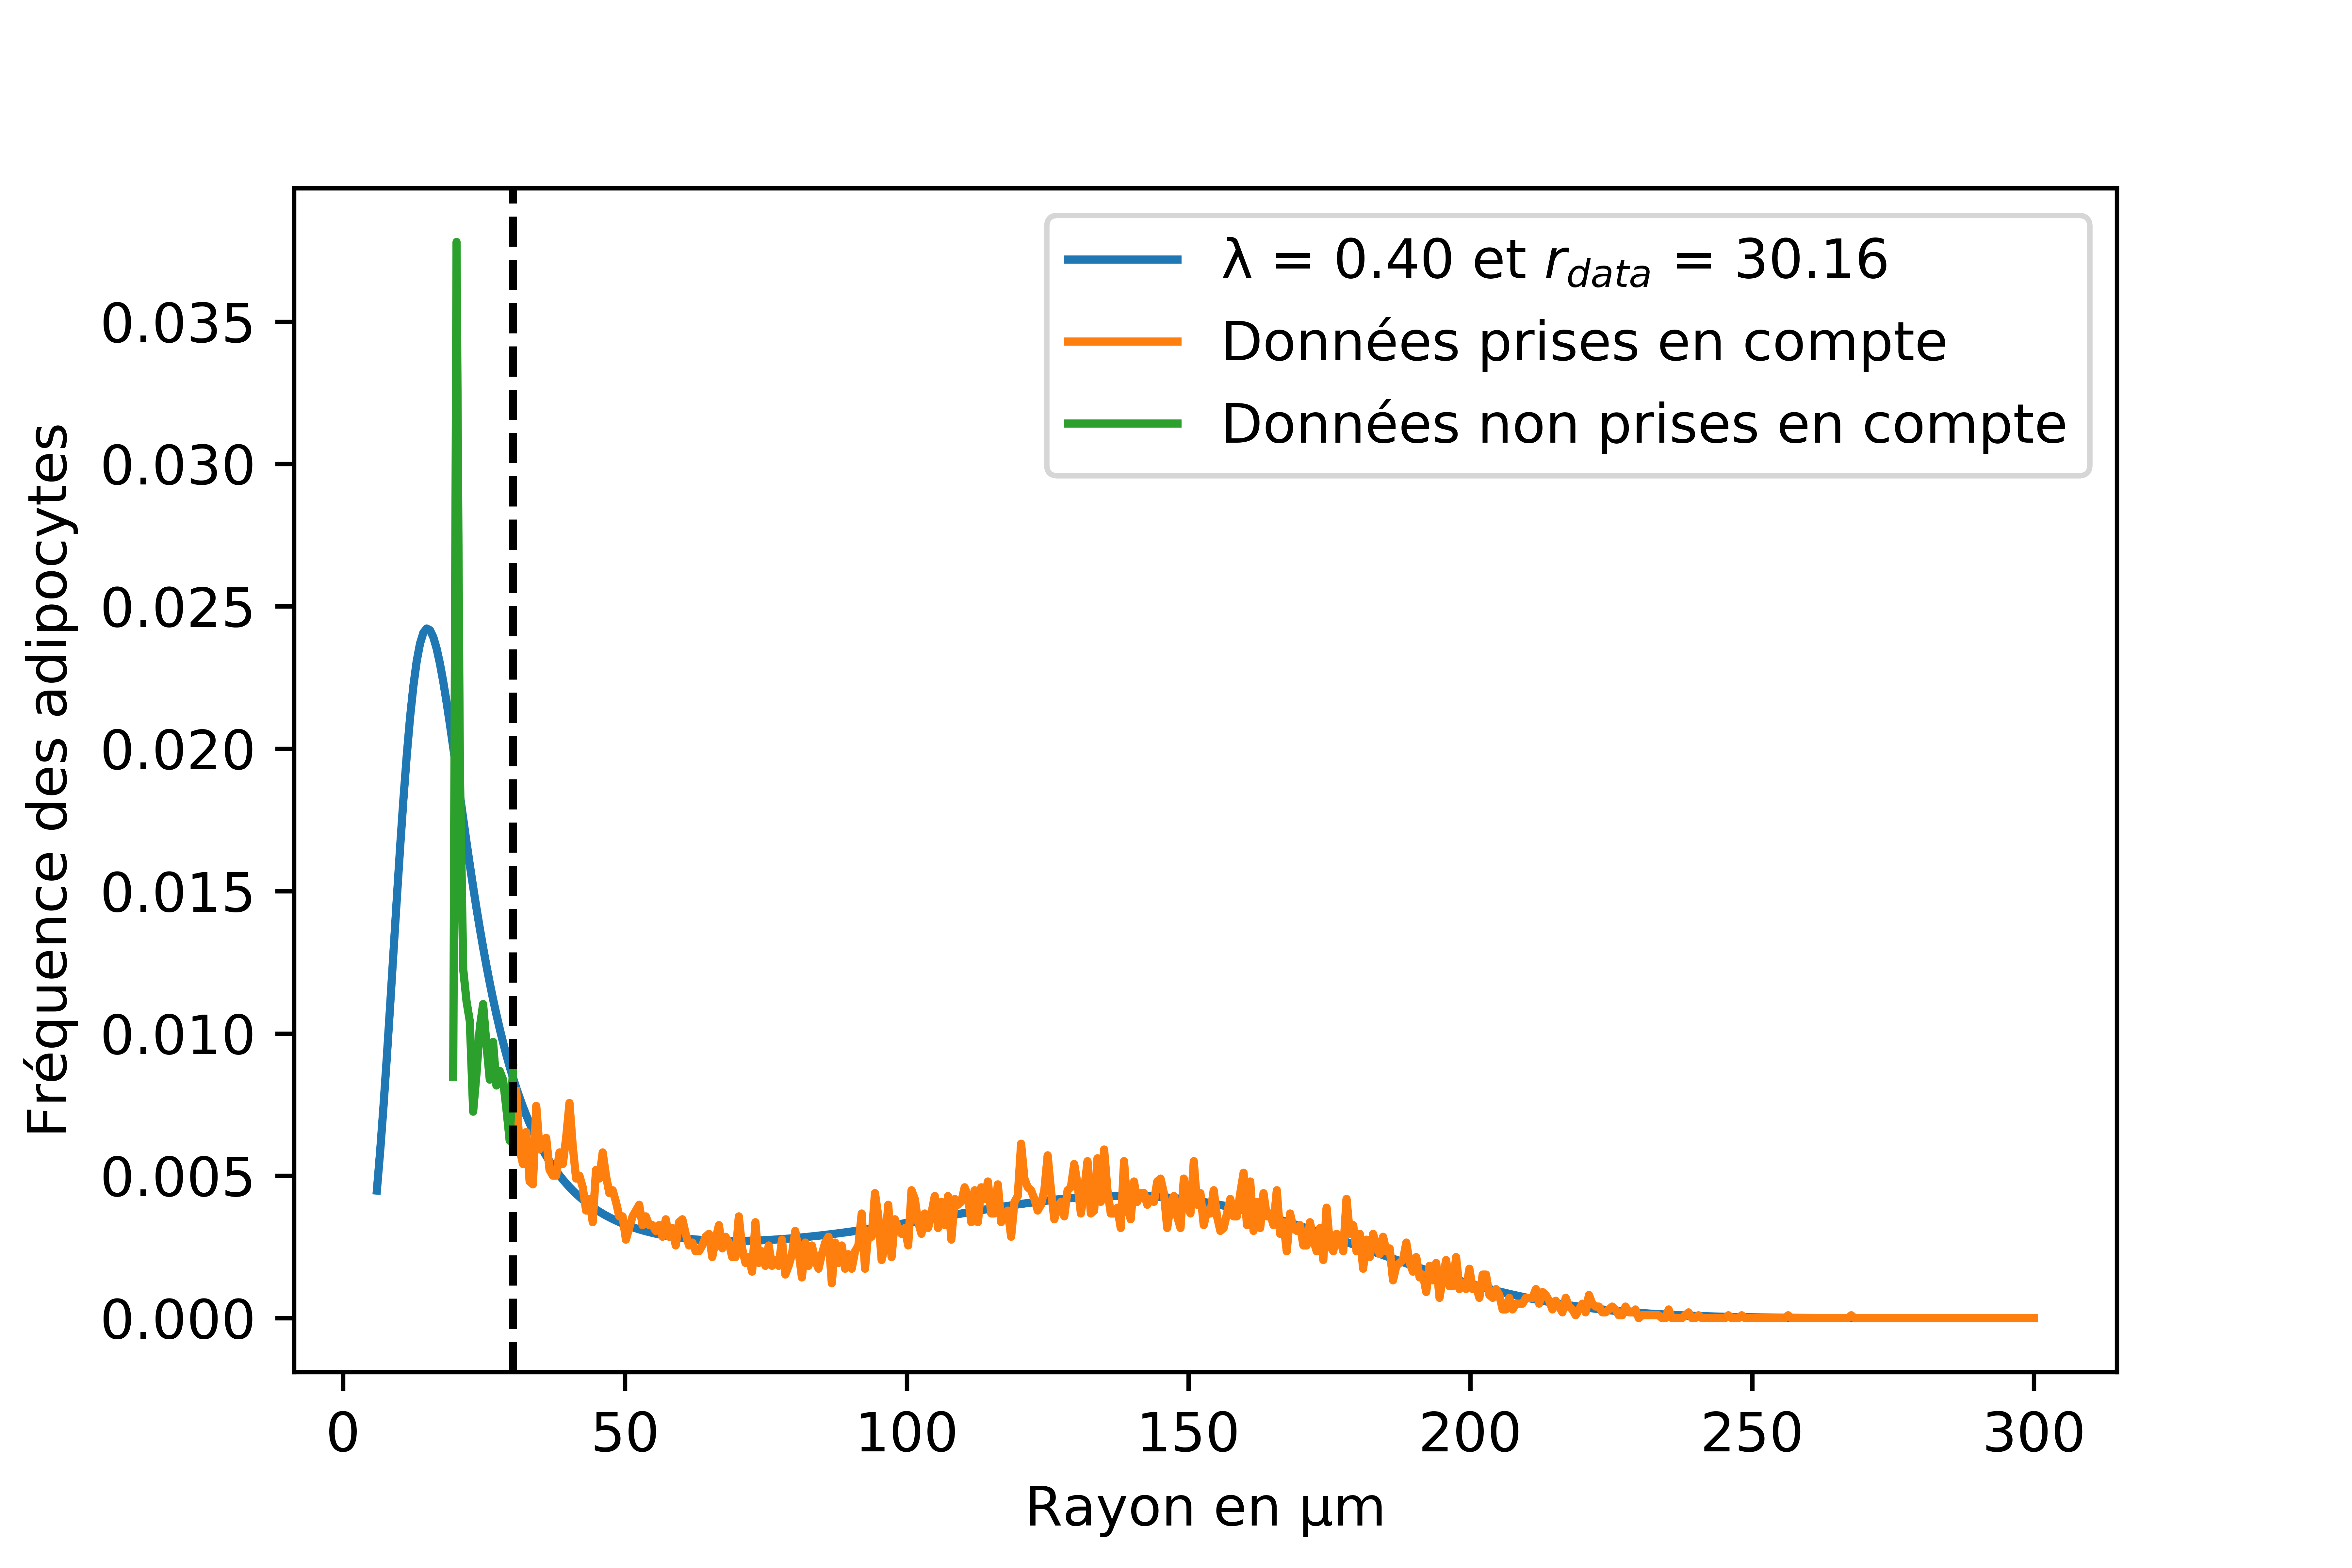
\includegraphics[scale=0.9]{Hys-D0-1-1}
\end{figure}

\begin{figure}[H]
\centering
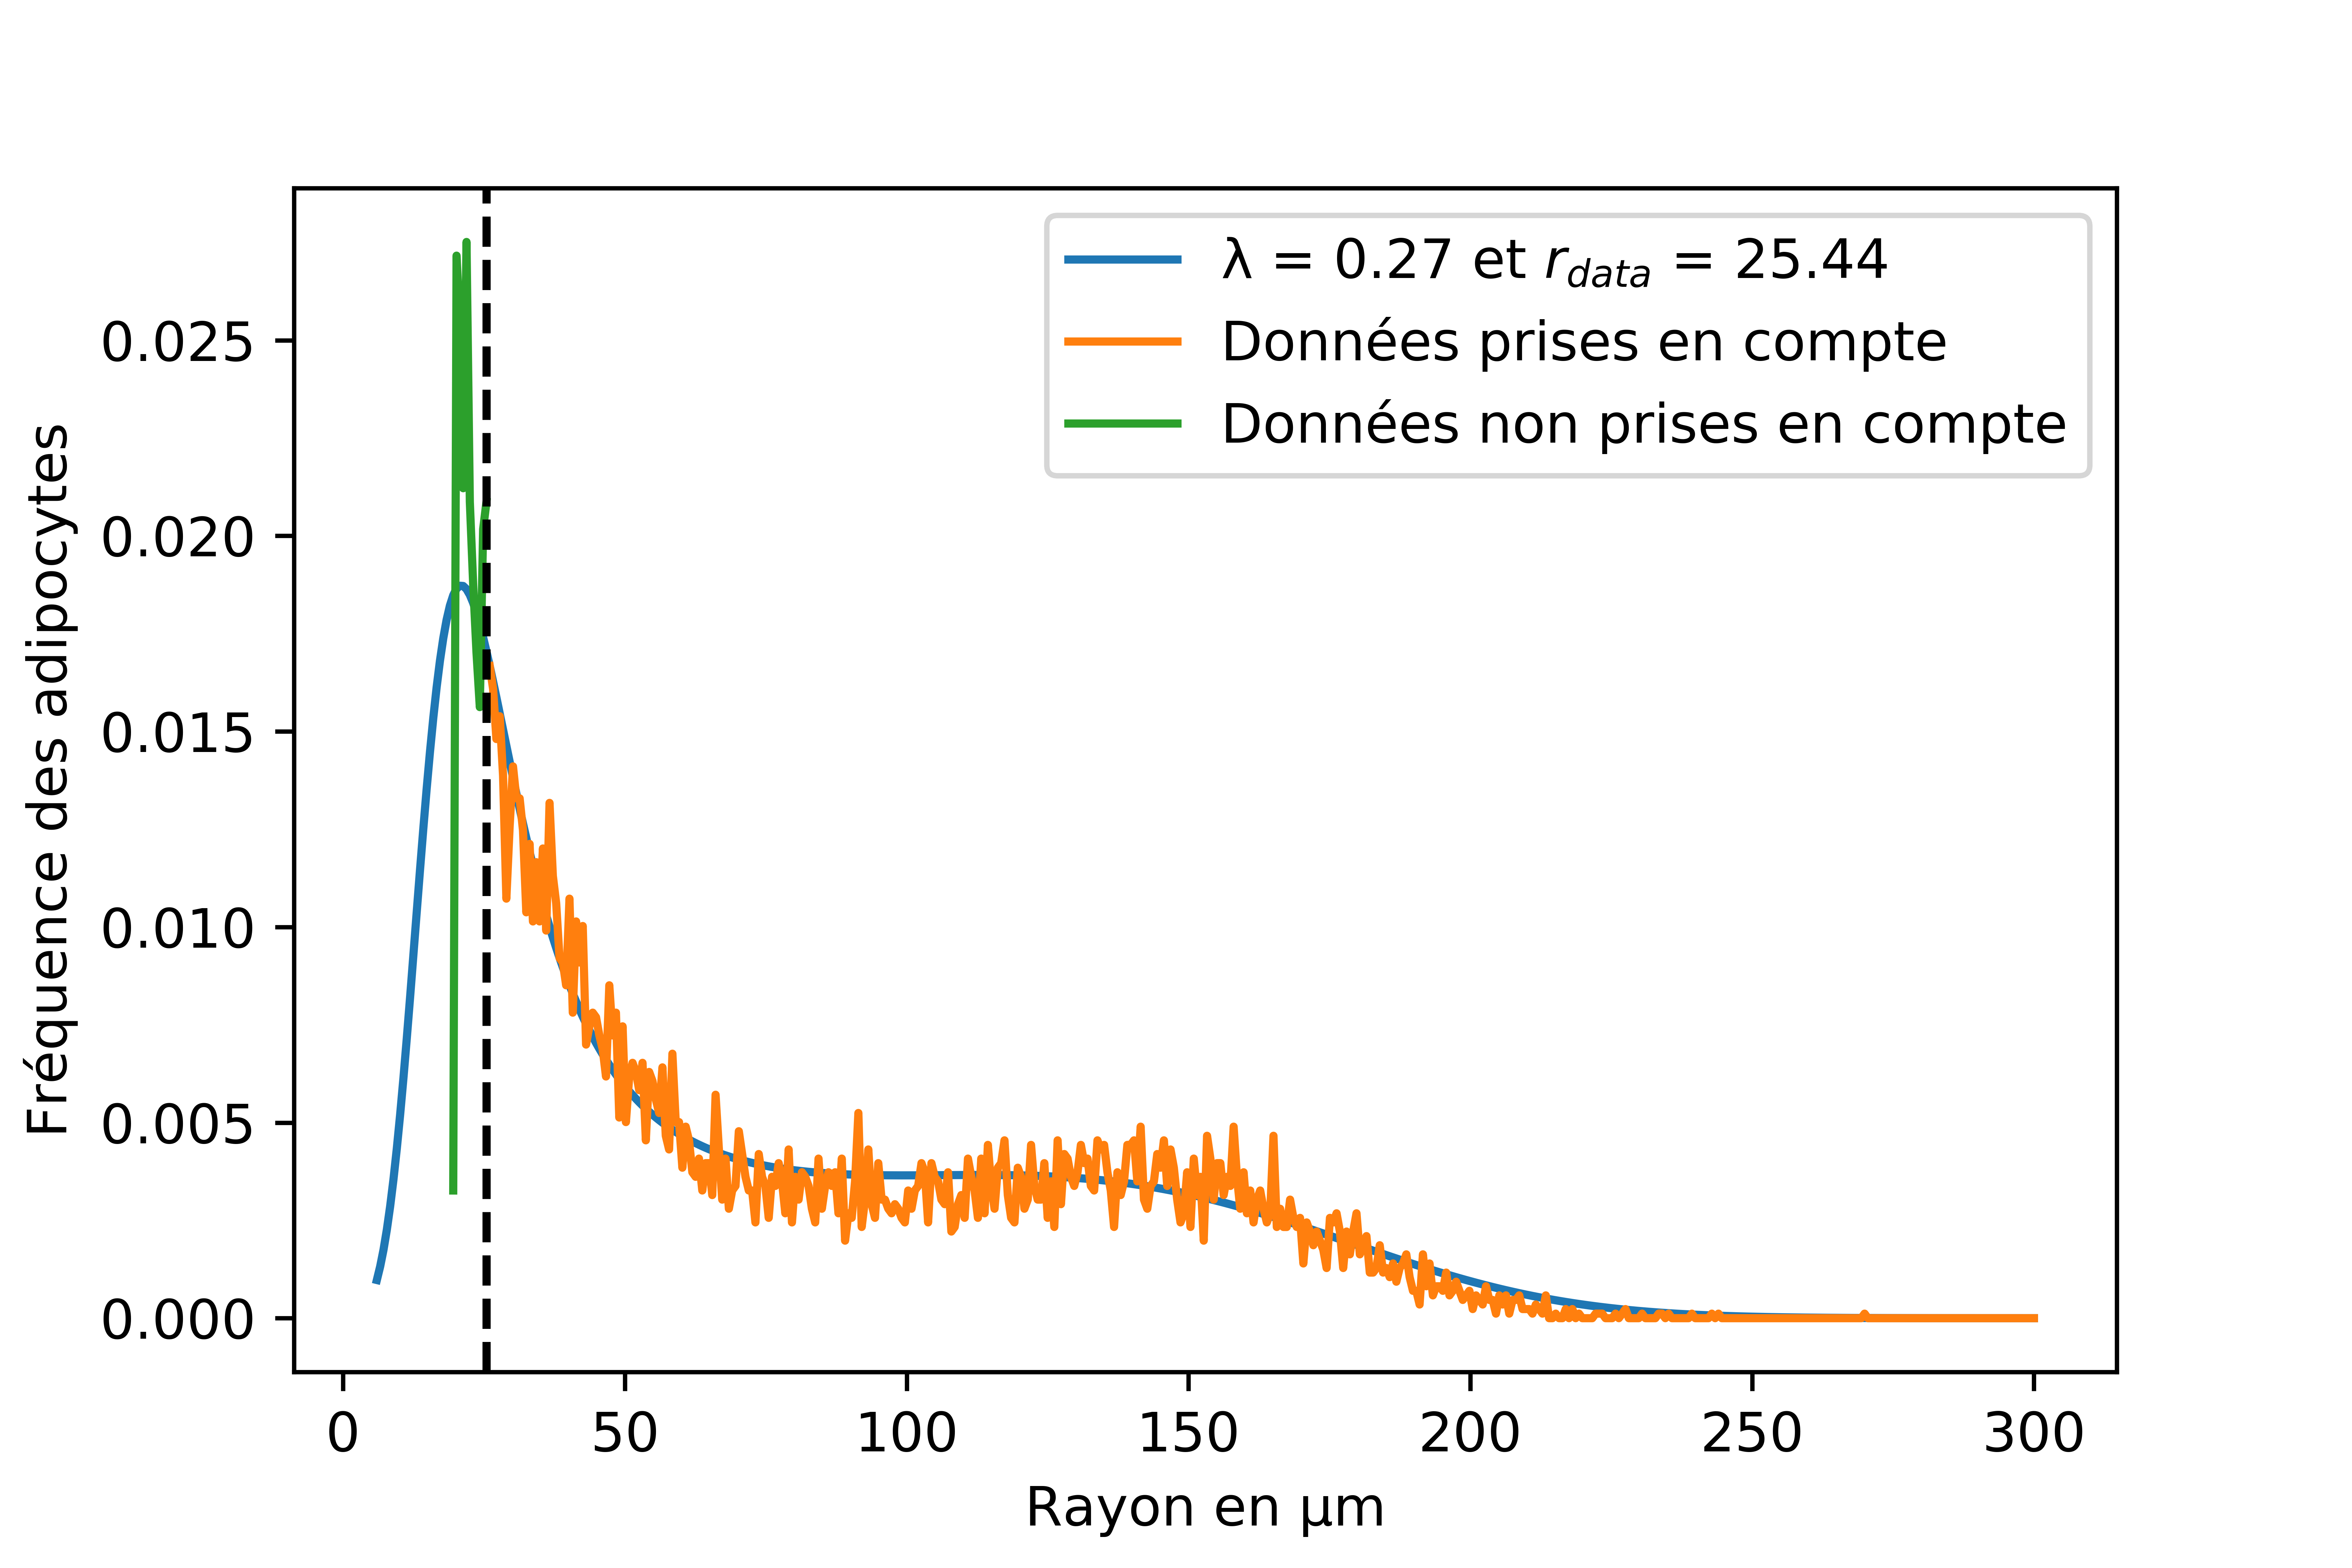
\includegraphics[scale=0.9]{Hys-D0-2-1}
\end{figure}

\begin{figure}[H]
\centering
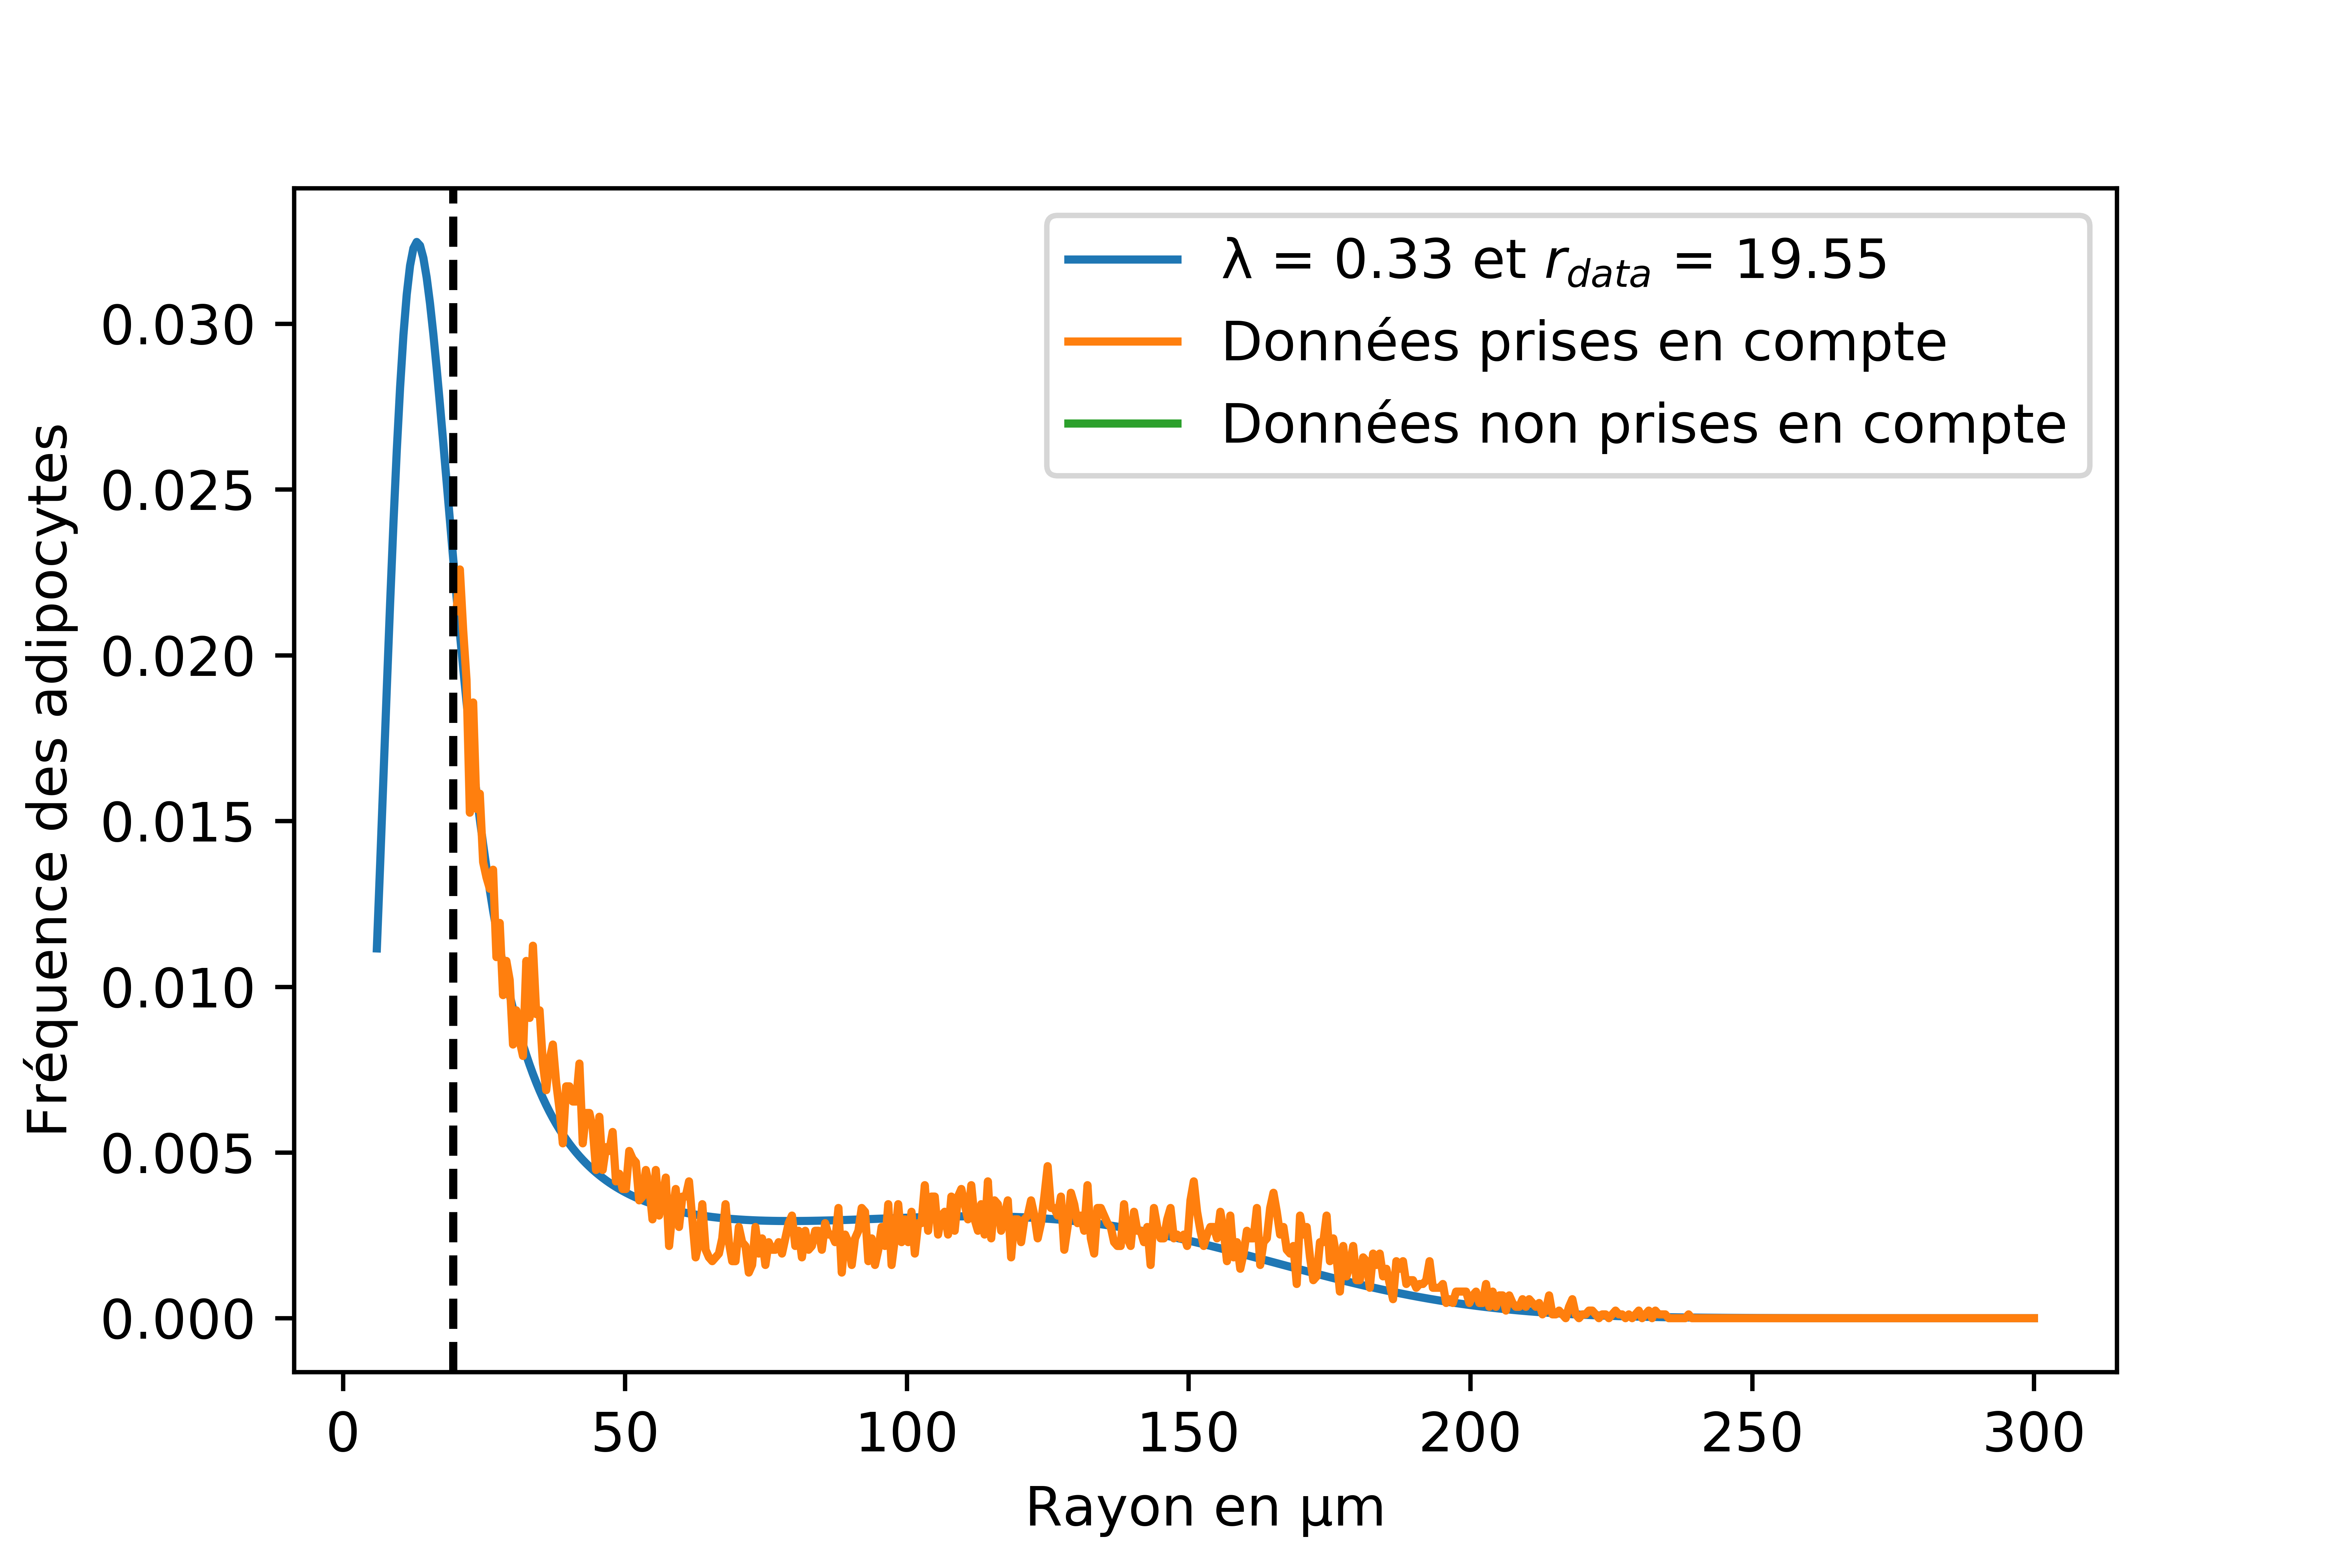
\includegraphics[scale=0.9]{Hys-D0-3-1}
\end{figure}

\begin{figure}[H]
\centering
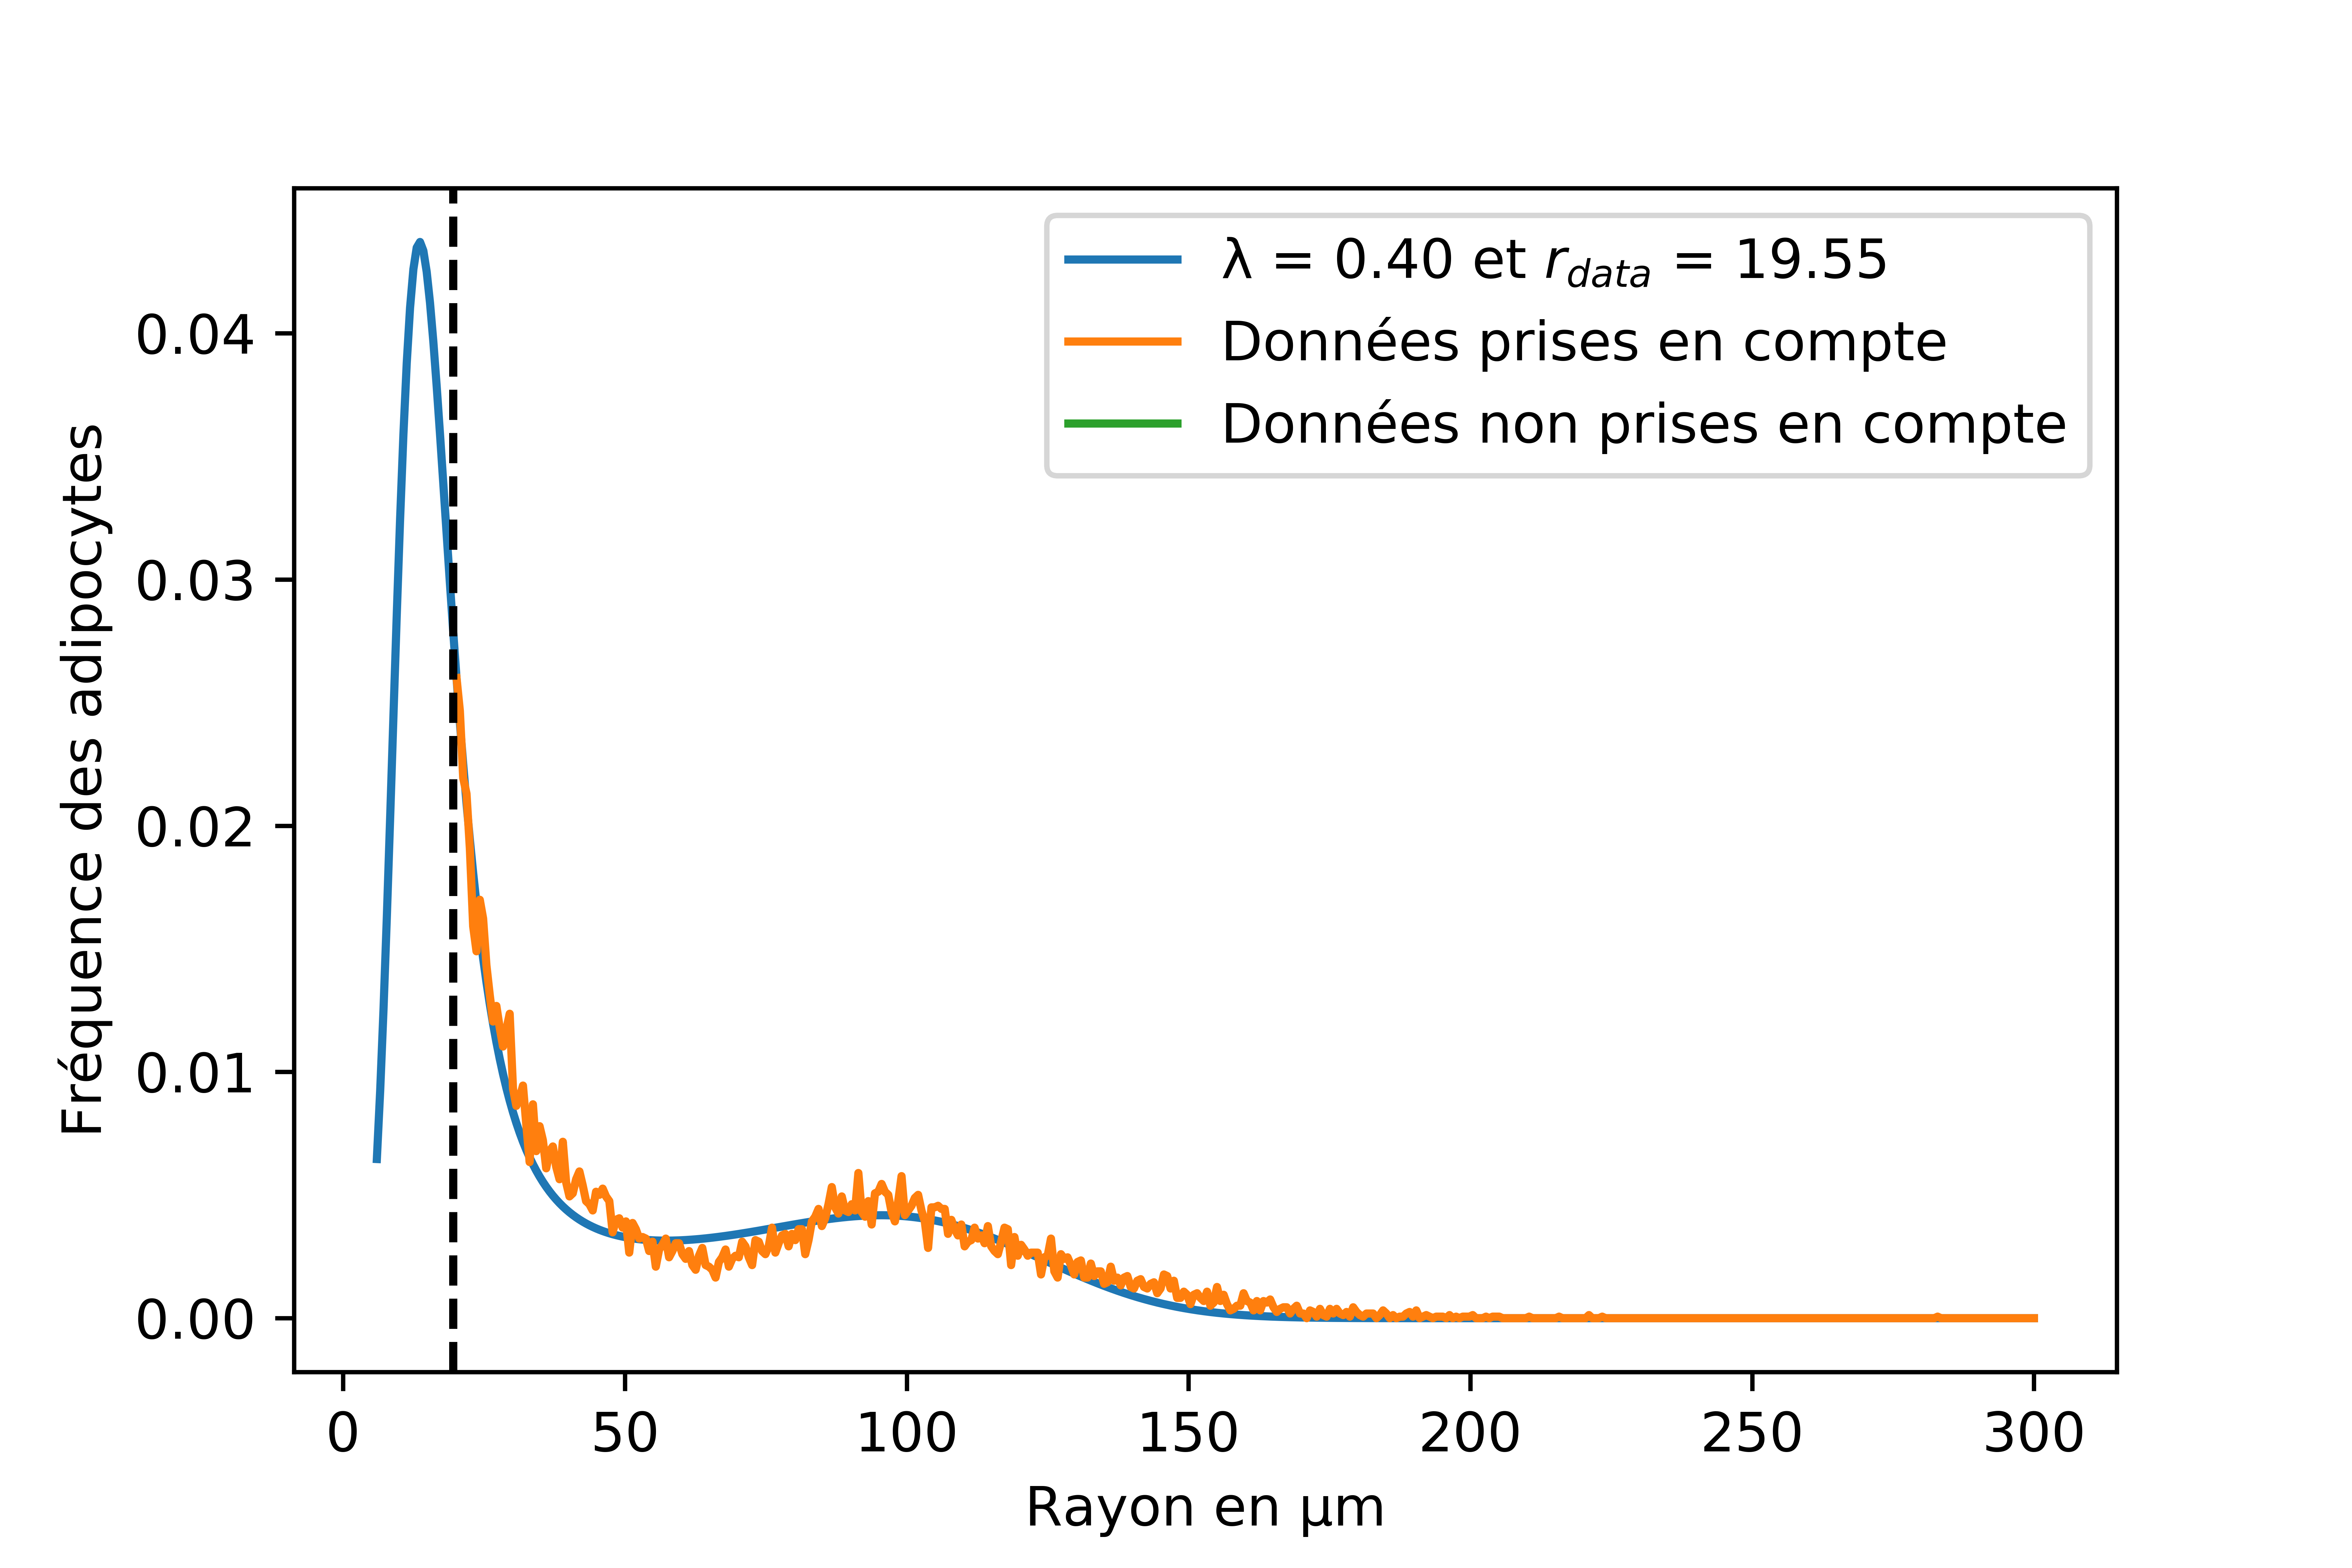
\includegraphics[scale=0.9]{Hys-D0-4-1}
\end{figure}

\section{Résultat d'algorithme PMCABC}\label{appendix:B}

\begin{figure}[H]
\centering
\includegraphics[scale=0.5]{abcpmc_6var_data}
\caption{Résultat de l'algorithme PMCABC sur une donnée expérimentale. On observe une erreur entre la moyenne de la distribution et le résultat du 'fit' pour certains paramètres.}
\end{figure}

\newpage

\bibliography{reference}
\bibliographystyle{plain}



\end{document}
